\documentclass[11pt,a4paper]{article}

% ============================================================================
% Packages
% ============================================================================
\usepackage[margin=2.4cm,top=2.6cm,bottom=2.6cm]{geometry}
\usepackage[T1]{fontenc}
\usepackage[utf8]{inputenc}
\usepackage{libertine}
\usepackage[libertine]{newtxmath}
\usepackage{microtype}
\usepackage{booktabs}
\usepackage{tabularx}
\usepackage{array}
\usepackage{multirow}
\usepackage{siunitx}
\usepackage{tikz}
\usepackage{pgfplots}
\usepackage{pgfplotstable}
\pgfplotsset{compat=1.18}
\usetikzlibrary{patterns,positioning,arrows.meta,calc,shapes.geometric,fit,backgrounds}
\usepackage[dvipsnames,table]{xcolor}
\usepackage[colorlinks=true,urlcolor=linkNavy,linkcolor=linkNavy,citecolor=black]{hyperref}
\usepackage{xurl}
\urlstyle{same}
\renewcommand{\UrlFont}{\small\rmfamily\itshape}
\emergencystretch=3em
\hbadness=10000
\vbadness=10000
\usepackage{enumitem}
\usepackage{titlesec}
\usepackage{fancyhdr}
\usepackage{parskip}
\usepackage{setspace}
\usepackage{caption}
\usepackage{endnotes}
% Redirect \footnote to \endnote (rev-3 post-publication cleanup).
% Footnote markers (superscripts) still appear in-line; clicking them in the PDF
% jumps to the consolidated Notes section before Appendix A. microtype's
% \footnote patch is disabled above so this redirection sticks.
\let\footnote=\endnote
\let\footnotemark=\endnotemark
\let\footnotetext=\endnotetext
\renewcommand{\enotesize}{\small}
\renewcommand\notesname{Notes}

% ============================================================================
% Palette & Style
% ============================================================================
\definecolor{inkBlack}{HTML}{1a1a1a}
\definecolor{paperCream}{HTML}{fbfaf5}
\definecolor{deepNavy}{HTML}{0d3b66}
\definecolor{linkNavy}{HTML}{1a4d7d}
\definecolor{accentOchre}{HTML}{c17817}
\definecolor{accentTerracotta}{HTML}{a34a28}
\definecolor{accentSage}{HTML}{6b8e5e}
\definecolor{accentPlum}{HTML}{6b3b63}
\definecolor{mutedSlate}{HTML}{4a5d6e}
\definecolor{softGrey}{HTML}{5a5a5a}
\definecolor{paleGrey}{HTML}{d8d6d0}
\definecolor{lightCream}{HTML}{f1efe8}

% Figure/section colors
\definecolor{chartA}{HTML}{0d3b66}
\definecolor{chartB}{HTML}{c17817}
\definecolor{chartC}{HTML}{6b8e5e}
\definecolor{chartD}{HTML}{a34a28}
\definecolor{chartE}{HTML}{6b3b63}
\definecolor{chartF}{HTML}{4a5d6e}
\definecolor{chartG}{HTML}{2e7d78}

\sisetup{group-separator={,},detect-weight=true,detect-family=true}

\titleformat{\section}{\Large\bfseries\color{deepNavy}}{\thesection.}{0.7em}{}
\titleformat{\subsection}{\large\bfseries\color{inkBlack}}{\thesubsection}{0.6em}{}
\titlespacing*{\section}{0pt}{1.6em}{0.8em}
\titlespacing*{\subsection}{0pt}{1.2em}{0.5em}

\captionsetup{font=small,labelfont={bf,color=deepNavy},labelsep=period,skip=6pt}
\renewcommand{\figurename}{Figure}

\pagestyle{fancy}
\fancyhf{}
\fancyhead[L]{\small\color{softGrey}\textsc{The AI Compute Build-Out, 2026--2030}}
\fancyhead[R]{\small\color{softGrey}\thepage}
\renewcommand{\headrulewidth}{0pt}
\fancyfoot{}

% Custom column types
\newcolumntype{R}[1]{>{\raggedleft\arraybackslash}p{#1}}
\newcolumntype{L}[1]{>{\raggedright\arraybackslash}p{#1}}

% Footnote styling (slight muting, narrower rule)
\renewcommand{\footnoterule}{\noindent\textcolor{paleGrey}{\rule{5cm}{0.4pt}}\vspace{4pt}}
\setlength{\footnotesep}{8pt}

% ============================================================================
% Title Page
% ============================================================================
\begin{document}
\pagestyle{empty}

\vspace*{3.5cm}
\begin{center}
{\color{softGrey}\small\textsc{A Data-Driven Survey}}

\vspace{0.6cm}
{\color{inkBlack}\fontsize{28pt}{34pt}\selectfont\bfseries The AI Compute Build-Out}

\vspace{0.3cm}
{\color{deepNavy}\Large\textit{Scale, capex, silicon, and counterparty geography, 2026--2030}}

\vspace{2.5cm}
\begin{tikzpicture}
\node[draw=paleGrey,line width=0.4pt,rounded corners=2pt,inner sep=14pt,
      text width=13cm,align=left,fill=lightCream] {%
\color{inkBlack}\small
At the end of Q2 2026, the six-tier framework places approximately \textbf{7.56~GW of
directly-disclosed operational AI compute} at Tier~1 (tier-clean; corresponding to
approximately \textbf{8.7~GW at facility power} and blended PUE~1.16), with an additional
0.20~GW of T6 analyst-inferred operational capacity (Voltage~Park, Together~AI). Announced
commitments through 2030 imply a \textbf{raw horizon of approximately 51.9~GW facility
power} across Western-aligned operators --- equivalent to approximately \textbf{50.6~GW
on the IT-load bridge}. Under our realization-probability framework (T1 at 100\% through
T6 at 25\%) the deterministic tier-weighted point estimate is approximately \textbf{36.8~GW
facility}; a 10,000-draw Monte Carlo that samples tier realization rates from Beta-fitted
distributions and applies the five stress scenarios (\S\ref{subsec:stress-matrix}) with
their prior probabilities produces a \textbf{median 2030 realized horizon of approximately
31.8~GW facility} with an \textbf{interdecile range of [24.6, 37.4]~GW} --- our
probability-honest central estimate. The \textbf{raw non-stretch horizon} (announced minus
T5 stretch targets) is approximately \textbf{45.2~GW facility}. The \textbf{conservative
case} raw (Tiers~1+2+3 only) is approximately \textbf{27.9~GW facility}; the \textbf{full-realization
ceiling} is approximately \textbf{55.3~GW facility}. The associated capital envelope is
approximately \textbf{\$1.2--1.5 trillion}, separately underwritten by approximately
\textbf{\$550~billion} in contracted remaining performance obligations (RPO) --- revenue
commitments that enable project-finance debt, not a funding channel in their own right.
A separate approximately \textbf{2.06~GW facility} sovereign-AI pipeline in the UAE,
Saudi Arabia, India, and the UK is reported as a sidebar. Every cited number is paired
with an evidence tier (T1--T6) and resolvable to a row in the companion
\texttt{row\_level\_audit.csv} shipped alongside this PDF.
};
\end{tikzpicture}

\vfill
{\color{softGrey}\small
Data cutoff: April 24, 2026\quad\textbullet\quad Publication: April 24, 2026 (revision 3)\\[2pt]
Primary data: Epoch AI, \emph{Frontier Data Centers} (snapshot 2026-04-24, incorporating the 2026-04-22 changelog revision to Stargate Abilene and the 2026-04-10 revision to Meta Prometheus).\footnote{Epoch AI, \emph{Frontier Data Centers} dataset and changelog, retrieved April 24, 2026. \url{https://epoch.ai/data/data-centers}. Methodology (\url{https://epoch.ai/data/data-centers-documentation}) documents that the dataset's \texttt{Power (MW)} field is total facility power (IT accelerators plus cooling, lighting, and conversion losses); cooling-model power estimates can in principle vary by up to a factor of 2 against ground truth, though Epoch's validation against known-capacity sites shows agreement within approximately 50\%; capital-cost estimates apply a uniform \$44~B/GW (\$30~B hardware + \$14~B infrastructure) and do not vary by site. These bands are consistent with our T2 realization-probability range of 80--95\% and the T3 range of 65--90\% and provide external validation for the six-tier prior framework.} Supplementary disclosures cited in footnotes throughout.\\[2pt]
\emph{Rev-3 changes (2026-04-24).} The physical denominator is standardized to \textbf{facility power} (matching Epoch's \emph{Frontier Data Centers} convention and the basis most relevant to grid interconnection and facility capex), with \textbf{IT-load-equivalent capacity} reported separately as a secondary bridge against chip-nameplate commitments. The PUE sensitivity table is now direction-correct (facility $\rightarrow$ IT rather than the reversed IT $\rightarrow$ facility of revision~2). The retired ``45.7~GW bear'' label is replaced with the \emph{raw non-stretch horizon} (announced minus T5 stretch targets, approximately 45.2~GW facility); this re-labeling reflects that the Monte Carlo p95 lies below this figure, so the prior ``bear'' terminology was structurally misleading. Figure~8 is rebuilt as two distinct charts: Figure~8A (capex bridge --- what the money physically purchases) and Figure~8B (financing bridge --- where the money comes from); the \$550B RPO is now handled in separate prose as revenue underwriting that enables the debt-financing channel, not as a funding channel in its own right. The T1 tier partition is corrected to 7.56~GW (tier-clean: Epoch 6.27 + neocloud directly-disclosed 1.29), with the 0.20~GW T6 analyst-inferred operational capacity (Voltage~Park, Together) held in T6 throughout the Monte Carlo and the rollup. Grid-region attribution is corrected: Meta Hyperion (Richland Parish, Louisiana) is MISO-South via Entergy, not ERCOT; xAI Colossus~2 (Memphis) is MISO via MLGW, not ERCOT.
}
\end{center}

\newpage
\pagestyle{fancy}
\setcounter{page}{2}

% ============================================================================
\section*{Contents}
\addcontentsline{toc}{section}{Contents}

\begin{spacing}{1.15}
\begin{tabular}{@{}R{0.6cm} L{11cm} R{1cm}@{}}
\textcolor{softGrey}{1.} & The scale of what is being built & 2 \\
\textcolor{softGrey}{2.} & Geographic concentration & 5 \\
\textcolor{softGrey}{3.} & The operators: who owns the horizon & 6 \\
\textcolor{softGrey}{4.} & The silicon: NVIDIA, Trainium, TPU, AMD, Broadcom, MTIA & 9 \\
\textcolor{softGrey}{5.} & The \$1.5 trillion question: where the money comes from & 11 \\
\textcolor{softGrey}{6.} & The counterparty graph & 14 \\
\textcolor{softGrey}{7.} & Execution risk: what breaks the build-out & 14 \\
\textcolor{softGrey}{8.} & Sovereign AI & 19 \\
\textcolor{softGrey}{9.} & Known unknowns & 20 \\
\textcolor{softGrey}{10.} & Conclusion & 22 \\
\textcolor{softGrey}{---} & Notes & 23 \\
\textcolor{softGrey}{A.} & Appendix: data sources and methodology & 28 \\
\textcolor{softGrey}{B.} & Appendix: row-level audit (summary) & 30 \\
\end{tabular}
\end{spacing}

\vspace{2cm}

% ============================================================================
\section{The scale of what is being built}
% ============================================================================

\textbf{Why we still estimate.} The relevant alternative to imperfect estimation is not perfect measurement; it is unstructured narrative. AI compute infrastructure moves through announcements, permits, grid queues, chip roadmaps, customer contracts, and project-finance vehicles faster than official statistics can capture. We therefore treat the 2030 build-out as a forecast object: uncertain, decomposable, and auditable. Every headline number in this paper is paired with an evidence tier (T1 Operational, T2 Physically-evidenced / under construction, T3 Firm commercial commitment, T4 Announced site-level plan, T5 LOI / stretch target, T6 Analyst inference) and a tier-default realization probability with per-row override. Appendix~B and the companion \texttt{row\_level\_audit.csv} provide the audit so the reader can reproduce every aggregate.

In Q2 2026, the operational AI compute fleet worldwide totals approximately \textbf{7.56~GW} tier-clean (T1; facility-equivalent approximately \textbf{8.7--9.0~GW} at blended PUE 1.16), with a further approximately \textbf{0.20~GW} T6-inferred from neocloud sources (Voltage Park, Together). The chip footprint is approximately \textbf{4.2~million H100-equivalent}.\footnote{Epoch AI, \emph{Frontier Data Centers} dataset, snapshot April 24, 2026, incorporating the 2026-04-22 changelog entry revising Stargate Abilene from a 600~MW April-1 milestone to ~200~MW actual operational. Epoch's ``Power (MW)'' field reports total facility power (GPUs + cooling + lighting + electrical losses); see \url{https://epoch.ai/data/data-centers-documentation}. H100-equivalent (H100e) normalizes GPU throughput by 8-bit operations per second relative to the NVIDIA H100 baseline.} Announced commitments through 2030 across the same operators --- hyperscalers, frontier labs, and the independent neoclouds --- imply a raw \textbf{51.9~GW facility} horizon across the Western-aligned operator set (\textbf{50.6~GW} IT-load bridge), with a further approximately \textbf{2.06~GW facility} in the sovereign-AI sidebar. Under tier-default probability weighting, the expected 2030 realization is approximately \textbf{36.8~GW facility}; the T1+T2+T3 conservative case is approximately \textbf{27.9~GW facility}; and the full-realization ceiling is approximately \textbf{55.3~GW facility}.

\textbf{The central fact} is that approximately 85\% of the 51.9~GW facility raw 2030 horizon is not yet operational (up from 84\% pre-rev-2, after the Stargate Abilene T1$\rightarrow$T2 reclassification); on a probability-weighted basis, the expected realization of approximately 36.8~GW facility leaves approximately 78\% still to build, and the Monte Carlo median of approximately 31.8~GW facility (\S\ref{subsec:monte-carlo}) implies that even under a probabilistically-honest reading approximately 75\% of the 2030 horizon remains to be built. The AI compute stack of the late 2020s is overwhelmingly a forward commitment, not an in-place fleet.

\begin{figure}[h]
\centering
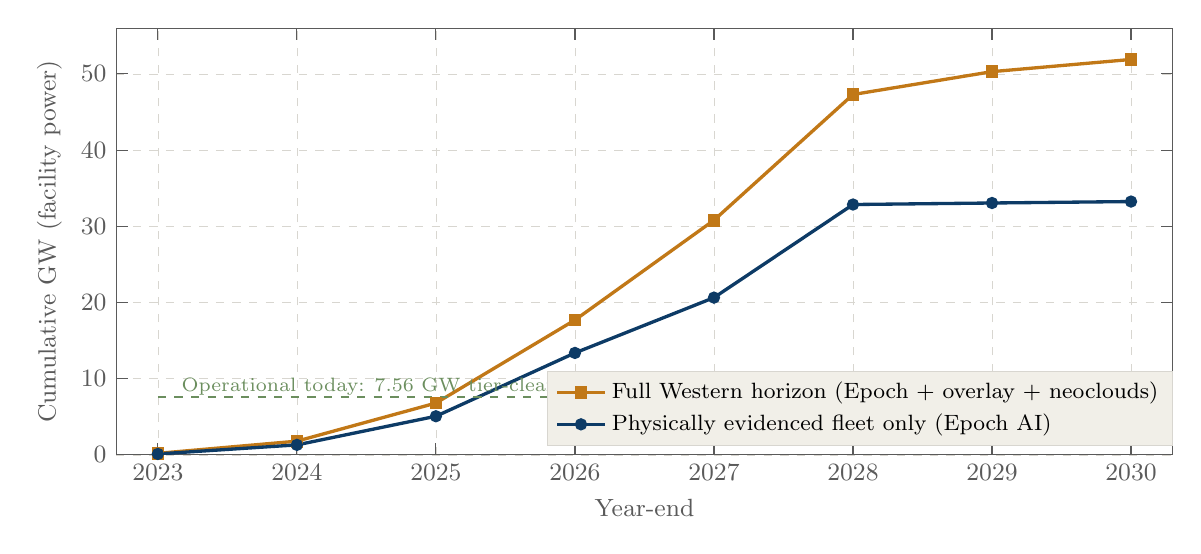
\begin{tikzpicture}
\begin{axis}[
  width=15cm, height=7cm,
  xlabel={Year-end}, ylabel={Cumulative GW (facility power)},
  xlabel style={font=\small,color=softGrey},
  ylabel style={font=\small,color=softGrey},
  xmin=2022.7, xmax=2030.3, ymin=0, ymax=56,
  xtick={2023,2024,2025,2026,2027,2028,2029,2030},
  xticklabel={\pgfmathprintnumber[1000 sep={}]{\tick}},
  xticklabel style={font=\small,color=softGrey},
  yticklabel style={font=\small,color=softGrey},
  axis line style={softGrey,thin},
  tick style={softGrey,thin},
  grid=major, grid style={paleGrey,dashed,very thin},
  legend style={at={(1.0,0.02)},anchor=south east,font=\footnotesize,draw=paleGrey,fill=lightCream},
  legend cell align={left},
]
% Full Western horizon (evidenced + overlay + neoclouds)
\addplot[color=accentOchre,line width=1.2pt,mark=square*,mark size=1.7pt,mark options={fill=accentOchre}] coordinates {
  (2023, 0.2) (2024, 1.8) (2025, 6.8) (2026, 17.7)
  (2027, 30.8) (2028, 47.3) (2029, 50.3) (2030, 51.9)
};
\addlegendentry{Full Western horizon (Epoch + overlay + neoclouds)}

% Epoch-evidenced only
\addplot[color=chartA,line width=1.2pt,mark=*,mark size=1.6pt] coordinates {
  (2023, 0.12) (2024, 1.31) (2025, 5.07) (2026, 13.38)
  (2027, 20.64) (2028, 32.86) (2029, 33.06) (2030, 33.25)
};
\addlegendentry{Physically evidenced fleet only (Epoch AI)}

% Horizontal reference line at today's tier-clean T1 operational level
\addplot[color=accentSage,dashed,line width=0.7pt,forget plot] coordinates {(2023,7.56) (2030,7.56)};
\node[color=accentSage,font=\scriptsize,anchor=west] at (axis cs:2023.1,9.0) {Operational today: 7.56 GW tier-clean (T1; ~8.7 GW facility-equiv at blended PUE 1.16)};
\end{axis}
\end{tikzpicture}
\caption{Cumulative AI compute capacity, 2023--2030. \textbf{Unit:} GW of facility power (rev-3 primary denominator; see \S\ref{subsec:power-units} for the IT-load bridge). \textbf{Included:} Epoch-tracked sites (blue); Class~A overlay + neocloud-ex-Epoch (ochre). \textbf{Excluded:} Class~B chip-procurement GW that deploys into existing shells; sovereign sidebar (reported separately in \S8). \textbf{Epistemic status:} blue is T1+T2 realized + T2/T3 near-term; ochre is the raw announced horizon (unweighted sum of T1--T5). The probability-weighted horizon (approximately 36.8~GW facility at 2030) sits between the two lines at the right edge. \textbf{What moves it:} stress scenarios A--D in \S\ref{subsec:stress-matrix} each shift the 2030 point by 1.5--8~GW.\protect\footnotemark}
\end{figure}
\footnotetext{Cumulative MW trajectory computed from Epoch AI's \emph{Frontier Data Centers} site-level event timelines, 2026-04-16 snapshot. Neocloud MW from operator primary filings: CoreWeave FY2025 10-K (filed 2026-02-26), Nebius Q4 FY2025 6-K (filed 2026-02-20), Applied Digital Q3 FY2026 10-Q (filed 2026-04-08).}

\subsection{Power units and PUE sensitivity}
\label{subsec:power-units}

Earlier drafts used ``IT-equivalent GW'' language too broadly. In this revision, we standardize the physical denominator to \emph{facility power}, matching Epoch AI's \emph{Frontier Data Centers} convention and the basis most relevant to grid interconnection and facility capex. We separately report IT-load-equivalent capacity for comparison against chip-nameplate commitments. The reader should keep five distinct power concepts in mind:

\begin{itemize}\itemsep2pt
\item \textbf{IT load} --- the nameplate power delivered to servers and accelerators. This is what chip vendors quote (e.g. ``1\,400 watts per Blackwell GB300'') and what cluster architects size racks against.
\item \textbf{Facility power} --- IT load multiplied by the Power Usage Effectiveness (PUE) ratio, which captures cooling, lighting, power-conversion losses, and auxiliary building load. Hyperscale AI campuses typically report PUE between 1.10 (aggressive liquid cooling) and 1.35 (air-cooled retrofits); older builds run 1.50--1.70.
\item \textbf{Grid interconnection capacity} --- the contracted-firm megawatt allocation at the substation. This can exceed facility power when operators reserve headroom for future phases, or fall short when utilities cap new connections.
\item \textbf{Cooling capacity} --- the thermal dissipation available at peak wet-bulb. In water-scarce locations (Arizona, West Texas), cooling-tower makeup water is itself a binding constraint and sites are rated in chiller tonnage as well as megawatts.
\item \textbf{Chip-commitment GW} --- a \emph{silicon} quantity reported by vendors (NVIDIA's ``10~GW'', Broadcom's ``10~GW XPU'') that expresses accelerator nameplate load \emph{independent of any specific site}. These numbers deploy \emph{into} physical shells already enumerated in the site-level census and must not be double-counted.
\end{itemize}

\textbf{Conversion policy.} Epoch AI's \emph{Frontier Data Centers} dataset reports \texttt{Power (MW)} as total facility power per its methodology documentation (GPUs, cooling, lighting, and conversion losses combined). The overlay YAML records \texttt{mw\_basis} and \texttt{pue\_assumed} per row: if \texttt{mw\_basis: facility} the published MW is used as-is; if \texttt{mw\_basis: IT} the figure is multiplied by the row's \texttt{pue\_assumed} to obtain facility power; if \texttt{mw\_basis: unknown} the paper default PUE~1.25 is applied. For Class~A Western overlay commitments, the per-row PUE values are 1.10 (Meta Hyperion, aggressive liquid cooling), 1.15 (OpenAI--Microsoft Fairwater), 1.18 (Anthropic--Azure), 1.20 (Anthropic--AWS), and 1.30 (xAI Colossus~2 Memphis, air-cooled retrofit). For neocloud operators, all material contributors (CoreWeave, Nebius, Nscale, Crusoe, Lambda, Applied Digital) already publish MW on facility basis per 10-K / 10-Q disclosure; only the three GPU-count-inferred operators (Fluidstack, Voltage Park, Together AI) carry \texttt{mw\_basis: IT} with PUE~1.25. Full per-row disclosure appears in Appendix~B.

\textbf{PUE sensitivity.} The facility-basis 51.9~GW point estimate maps to \emph{IT-load-equivalent} capacity by dividing by the blended PUE; this is the relevant bridge for comparison against chip-nameplate aggregates (NVIDIA's 10~GW LOI, Broadcom's 10~GW XPU commitment).

\begin{table}[h]
\centering
\small
\begin{tabular}{@{}lrr@{}}
\toprule
\textbf{PUE assumption} & \textbf{Western 2030 GW (IT-load equivalent)} & \textbf{Change vs.\ facility baseline} \\
\midrule
1.10 (aggressive liquid cooling, new builds) & 47.2 & $-$9.1\% \\
1.20 (paper blended central; Epoch baseline) & 43.3 & $-$16.6\% \\
1.30 (typical hyperscale air/hybrid) & 39.9 & $-$23.1\% \\
1.50 (older hyperscale retrofits) & 34.6 & $-$33.3\% \\
1.60 (legacy colocation) & 32.5 & $-$37.5\% \\
\bottomrule
\end{tabular}
\caption{IT-load-equivalent capacity mapped from the 51.9~GW facility-basis Western 2030 horizon under five PUE assumptions. The central IT-load bridge at blended PUE~1.20 is approximately 43~GW, consistent with the overlay-YAML's direct IT-basis rollup of 50.6~GW (which mixes IT-declared rows with facility-declared rows that pass through 1:1). Readers comparing against utility-contracted-MW or grid-interconnect datasets (EIA~861, FERC queue) should use the facility figures; readers comparing against chip-nameplate aggregates (NVIDIA/Broadcom ``X~GW'' silicon commitments) should use the IT-load equivalents.}
\end{table}

At facility baseline 51.9~GW, the IT-load-equivalent capacity falls in the range roughly $[39, 47]$~GW depending on PUE, with a central IT-equivalent of approximately 43~GW at blended PUE~1.20. This is the IT-load bridge referenced throughout the paper. The PUE range 1.10--1.35 captures where every currently-announced frontier-AI campus operates at scheduled commissioning.

\subsection{The two axes: physical capacity and compute capacity}

Physical capacity is measured in gigawatts of IT-relevant power --- the binding constraint that determines how much grid connection, land, water, and permits are required. Compute capacity is measured in H100-equivalents --- the relevant quantity for training and serving frontier models. The two grow at different rates because chip-generation improvements drop roughly every two years, each generation delivering substantially more 8-bit throughput per watt than the last.\footnote{NVIDIA Corporation, GTC 2026 keynote, March 2026, detailing the Blackwell~$\rightarrow$~Rubin~$\rightarrow$~Feynman cadence. \url{https://www.nvidia.com/en-us/events/gtc/}}

\begin{figure}[h]
\centering
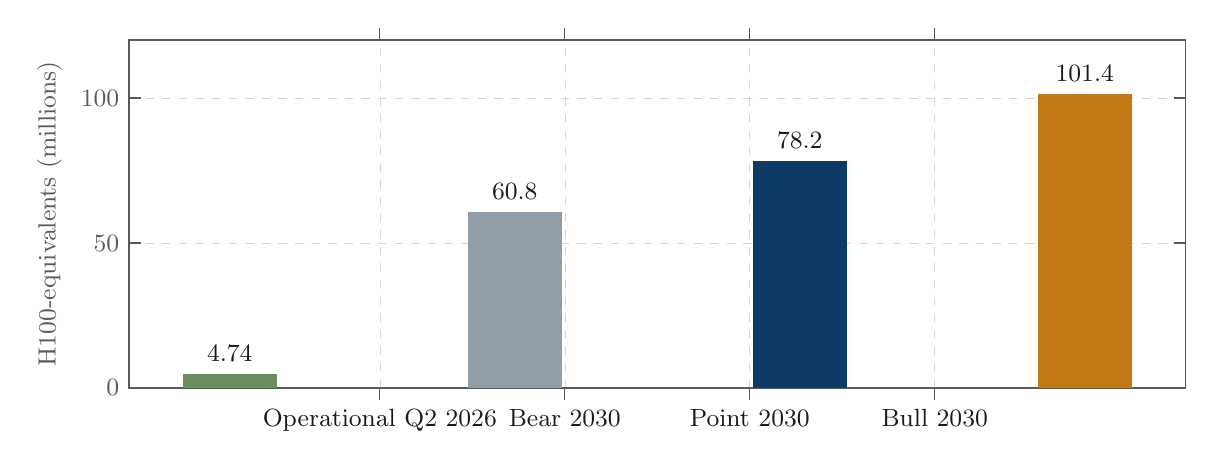
\begin{tikzpicture}
\begin{axis}[
  width=15cm, height=6cm,
  ybar,
  bar width=1.2cm,
  enlarge x limits=0.18,
  xtick={0,1,2,3},
  xticklabels={Operational Q2 2026,Bear 2030,Point 2030,Bull 2030},
  xticklabel style={font=\small,color=inkBlack},
  ylabel={H100-equivalents (millions)},
  ylabel style={font=\small,color=softGrey},
  yticklabel style={font=\small,color=softGrey},
  ymin=0, ymax=120,
  xmin=-0.6, xmax=3.6,
  nodes near coords,
  nodes near coords style={font=\small\bfseries,color=inkBlack,anchor=south,yshift=1pt},
  axis line style={softGrey,thin},
  tick style={softGrey,thin},
  grid=major, grid style={paleGrey,dashed,very thin},
]
\addplot[fill=accentSage,draw=none] coordinates {(0,4.74)};
\addplot[fill=chartF!60,draw=none] coordinates {(1,60.8)};
\addplot[fill=chartA,draw=none] coordinates {(2,78.2)};
\addplot[fill=accentOchre,draw=none] coordinates {(3,101.4)};
\end{axis}
\end{tikzpicture}
\caption{Compute capacity measured in H100-equivalents, today vs.\ 2030 Western horizon. Point estimate of 78.2M H100e (revised 2026-04-24 from 78.4M after the Epoch 2026-04-10 Meta Prometheus adjustment from 1.2M to 1.0M) implies a \textbf{18.6-fold expansion} of frontier-training compute between operational-today 4.2M H100e and the 2030 horizon, versus the 6.5-fold expansion in physical GW. Bear and bull bounds reflect sensitivity to NVIDIA Rubin Ultra and Feynman generational uplift, AWS Trainium3 per-chip improvement, and the realisation of Meta's Hyperion stretch target.\protect\footnotemark}
\end{figure}
\footnotetext{Epoch layer (46.35M H100e at 33.23 GW full buildout) taken directly from Epoch AI \emph{Frontier Data Centers} timeline H100e field. Class~A overlay and neocloud-ex-Epoch layers computed using (chip-family $\times$ end-of-timeline year) density, anchored on Epoch's current per-family density (Microsoft NVIDIA Blackwell sites: 910 H100e/MW; AWS Trainium~2 sites: 628 H100e/MW; Google TPU v5p/v6 sites: 475 H100e/MW) and the published chip-generation roadmap. \textbf{Basis note (rev-3):} all per-MW densities above are quoted per \emph{IT-MW} (Epoch internal convention). The facility-MW equivalent at blended PUE~1.20 is approximately 17\% lower --- e.g.\ the blended Epoch-weighted 1{,}388 H100e/IT-MW corresponds to approximately 1{,}157 H100e/facility-MW. Chip counts are basis-invariant (the chips are deployed regardless of denominator); only the denominator changes.}

Expressed differently: under the base silicon-uplift assumption, the industry is building approximately \textbf{six times as many watts of AI compute capacity by 2030 as are operational today, and roughly sixteen times as many H100-equivalent chips}. The conservative silicon case yields approximately 12$\times$ on H100e and the aggressive case approximately 22$\times$ (see \S\ref{subsec:h100e-sensitivity}). Chip-generation progress is contributing as much compute expansion as physical build-out across the base and aggressive cases. Any analysis that holds silicon constant understates the 2030 compute base by a factor of two to three.

\subsection{Operator concentration is extreme}

The 8.2 GW operational today is held by approximately ten entities. Within the United States, which accounts for \textbf{6.47 GW of the current 6.67 GW Epoch-evidenced floor (97\%)},\footnote{Author calculation from Epoch AI \emph{Frontier Data Centers}, 2026-04-16 snapshot. All non-US Epoch sites are in China (Alibaba Zhangbei, 203~MW current).} six counterparties each command more than 400 MW of operational capacity: Amazon (1{,}433 MW, including the 1.09 GW Anthropic-dedicated New Carlisle campus\footnote{Epoch AI \emph{Frontier Data Centers}, site entry ``Anthropic-Amazon New Carlisle'', current power 1{,}092~MW; Amazon Web Services and Anthropic, \emph{Announcement of Project Rainier}, November 13, 2024. \url{https://press.aboutamazon.com/2024/11/amazon-and-anthropic-deepen-strategic-collaboration}}), Microsoft (1{,}251 MW), Google (956 MW), Meta (729 MW), Oracle (590 MW, entirely OpenAI Stargate Abilene), and xAI (425 MW at the original Memphis Colossus).\footnote{Ownership and attribution per Epoch AI site-level tags; Oracle Stargate Abilene attribution confirmed in OpenAI, \emph{Announcing the Stargate Project}, January 21, 2025, \url{https://openai.com/index/announcing-the-stargate-project}, with Oracle, \emph{Q3 FY2026 earnings prepared remarks}, March 10, 2026.} The frontier neoclouds --- CoreWeave, Nebius, Crusoe, Lambda, Fluidstack, Nscale, Applied Digital, Voltage Park, Together AI --- collectively hold approximately 1.49 GW of operational capacity outside the Epoch-tracked set.\footnote{CoreWeave FY2025 10-K, operational capacity disclosure; Nebius Q4 FY2025 shareholder letter filed on 6-K, 2026-02-20; Applied Digital Q3 FY2026 10-Q, 2026-04-08; Crusoe, Nscale, Lambda, Fluidstack, Voltage Park, Together AI aggregated from press disclosures cited in Appendix~A.}

By 2030 on an announced-horizon basis, the same operator set expands to approximately \textbf{51.9~GW facility} aggregate (raw; 50.6~GW IT-load bridge); to approximately \textbf{36.8~GW facility} probability-weighted; and to approximately \textbf{27.9~GW facility} under the conservative T1+T2+T3 case. The three largest operators (Microsoft, Amazon-including-Anthropic, OpenAI-Stargate) each individually carry more than 10~GW of announced buildout --- with Amazon/Anthropic's 12.9~GW dominated by the T4 Anthropic expansion announcement (3.17~GW incremental at 72\% realization), OpenAI/Stargate's 10.6~GW dominated by T4 Stargate 8 sites (at a blended 70\% realization because Stargate is capex-secured but grid-interconnection-constrained), and Microsoft's 5.3~GW sitting largely at T2 (Fairwater construction visible) with realization probabilities near 85\%.

\begin{figure}[h]
\centering
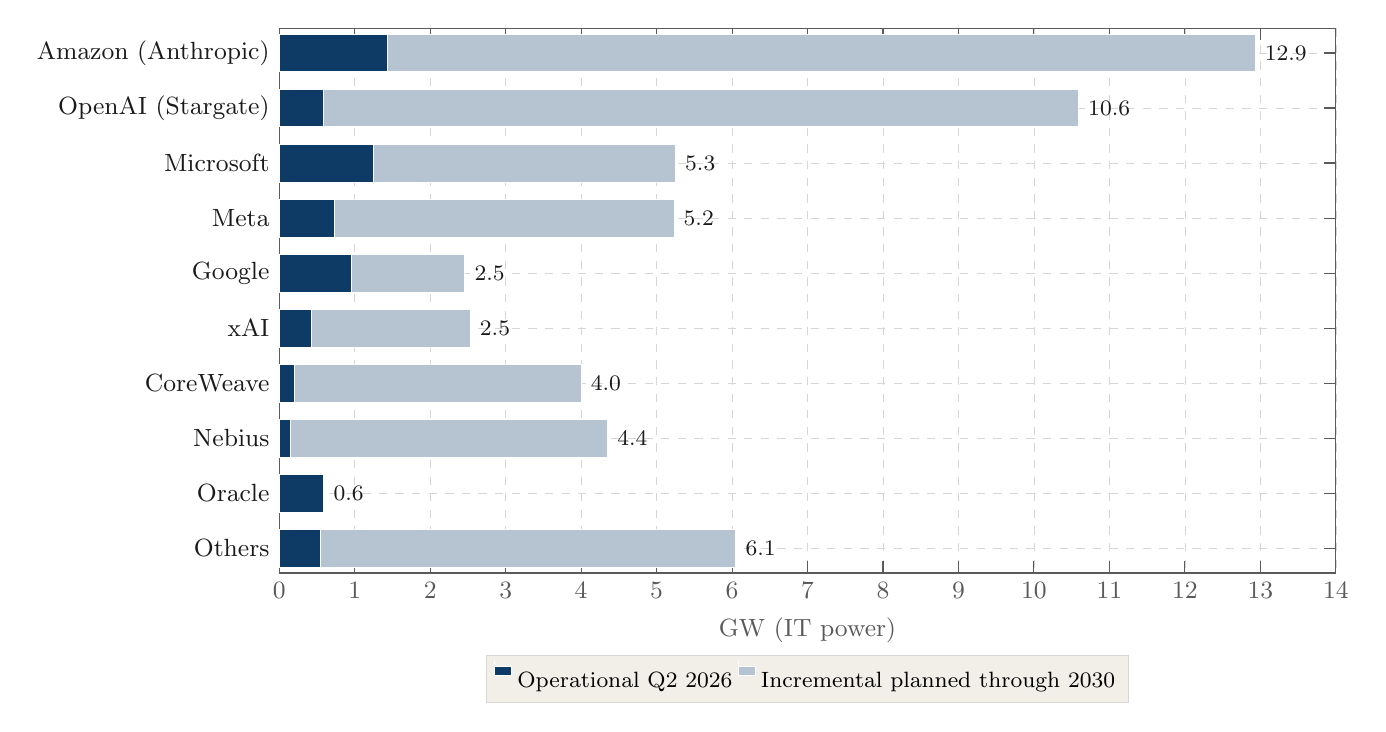
\begin{tikzpicture}
\begin{axis}[
  width=15cm, height=8.5cm,
  xbar stacked,
  bar width=0.48cm,
  enlarge y limits=0.05,
  symbolic y coords={Amazon,OpenAI,Microsoft,Meta,Google,xAI,CoreWeave,Nebius,Oracle,Others},
  ytick=data,
  yticklabels={Amazon (Anthropic),OpenAI (Stargate),Microsoft,Meta,Google,xAI,CoreWeave,Nebius,Oracle,Others},
  y dir=reverse,
  xlabel={GW (IT power)},
  xlabel style={font=\small,color=softGrey},
  yticklabel style={font=\small,color=inkBlack},
  xticklabel style={font=\small,color=softGrey},
  xmin=0, xmax=14,
  axis line style={softGrey,thin},
  tick style={softGrey,thin},
  grid=major, grid style={paleGrey,dashed,very thin},
  legend style={at={(0.5,-0.15)},anchor=north,font=\footnotesize,draw=paleGrey,fill=lightCream,legend columns=2},
  legend cell align={left},
]
% Segment 1: operational
\addplot+[fill=chartA,draw=white,line width=0.3pt,ybar legend] coordinates {
  (1.43,Amazon) (0.59,OpenAI) (1.25,Microsoft) (0.73,Meta) (0.96,Google)
  (0.43,xAI) (0.20,CoreWeave) (0.15,Nebius) (0.59,Oracle) (0.55,Others)
};
\addlegendentry{Operational Q2 2026}
% Segment 2: incremental
\addplot+[fill=chartA!30,draw=white,line width=0.3pt,ybar legend] coordinates {
  (11.5,Amazon) (10.0,OpenAI) (4.0,Microsoft) (4.5,Meta) (1.5,Google)
  (2.1,xAI) (3.8,CoreWeave) (4.2,Nebius) (0.0,Oracle) (5.5,Others)
};
\addlegendentry{Incremental planned through 2030}
% Total labels at bar ends
\node[font=\footnotesize,color=inkBlack,anchor=west] at (axis cs:12.93,Amazon)  {12.9};
\node[font=\footnotesize,color=inkBlack,anchor=west] at (axis cs:10.59,OpenAI)  {10.6};
\node[font=\footnotesize,color=inkBlack,anchor=west] at (axis cs:5.25,Microsoft){5.3};
\node[font=\footnotesize,color=inkBlack,anchor=west] at (axis cs:5.23,Meta)     {5.2};
\node[font=\footnotesize,color=inkBlack,anchor=west] at (axis cs:2.46,Google)   {2.5};
\node[font=\footnotesize,color=inkBlack,anchor=west] at (axis cs:2.53,xAI)      {2.5};
\node[font=\footnotesize,color=inkBlack,anchor=west] at (axis cs:4.00,CoreWeave){4.0};
\node[font=\footnotesize,color=inkBlack,anchor=west] at (axis cs:4.35,Nebius)   {4.4};
\node[font=\footnotesize,color=inkBlack,anchor=west] at (axis cs:0.59,Oracle)   {0.6};
\node[font=\footnotesize,color=inkBlack,anchor=west] at (axis cs:6.05,Others)   {6.1};
\end{axis}
\end{tikzpicture}
\caption{Operator-level operational vs.\ announced-incremental capacity through 2030. ``Amazon (Anthropic)'' aggregates AWS-owned sites hosting Anthropic workloads under Project Rainier and the April 2026 expansion; ``OpenAI (Stargate)'' aggregates Oracle-operated, SoftBank-MGX-financed sites. Neocloud figures for CoreWeave and Nebius are operator-contracted capacity under long-dated take-or-pay with named hyperscaler or lab customers. ``Others'' includes Applied Digital, Crusoe, Nscale, Lambda, Fluidstack, Together AI, Voltage Park, and non-Epoch long-tail operators.\protect\footnotemark}
\end{figure}
\footnotetext{Operator-level aggregation from Epoch AI site-level owner attribution plus operator primary disclosures. Amazon incremental through 2030 reflects Anthropic's April 20, 2026 announcement of ``up to 5~GW of new capacity'' and existing Project Rainier buildout. See Anthropic and Amazon, \emph{Anthropic and Amazon expand collaboration for up to 5 gigawatts of new compute}, April 20, 2026, \url{https://www.anthropic.com/news/anthropic-amazon-compute}.}

% ============================================================================
\section{Geographic concentration}
% ============================================================================

The AI compute build-out is strikingly geographically concentrated. Of the 33.2 GW of Epoch-evidenced sites at scheduled full buildout, approximately \textbf{85\% sit in the continental United States} and approximately \textbf{60\% sit in just five states}: Texas, Wisconsin, Ohio, Mississippi, and Louisiana. Outside the United States, the largest clusters are in Norway (Microsoft-Nscale Narvik), the United Kingdom (Microsoft Loughton, CoreWeave London, UK AI Growth Zones), Ireland (Microsoft Dublin), Saudi Arabia (HUMAIN-AMD, xAI-HUMAIN), and the United Arab Emirates (G42-Khazna for Microsoft, Stargate UAE).

\subsection{The Texas--Ohio--Wisconsin triangle}

Three adjacent US grid footprints host the majority of the Western 2030 horizon. The ERCOT (Texas) system hosts OpenAI Stargate Abilene and Shackelford, Meta's Temple campus, Anthropic-Fluidstack Texas, and multiple secondary sites. The MISO (Midwest + South) system hosts Microsoft Fairwater Wisconsin (3.3 GW at full buildout, the single largest planned AI site worldwide\footnote{Epoch AI \emph{Frontier Data Centers}, site entry ``Microsoft Fairwater Wisconsin'', full-buildout power 3{,}328~MW; Microsoft, \emph{Inside the world's most powerful AI datacenter}, September 18, 2025, \url{https://news.microsoft.com/source/features/ai/inside-the-worlds-most-powerful-ai-datacenter/}.}), Anthropic-Amazon New Carlisle (Ohio), Meta Hyperion (Richland Parish, Louisiana --- MISO-South via Entergy Louisiana, not ERCOT), xAI Colossus~2 (Memphis, Tennessee --- MISO via MLGW, not ERCOT), and QTS Cedar Rapids (Iowa). Northern Virginia --- historically the dominant commercial data-centre cluster in the world --- hosts a comparatively small share of the named AI-frontier pipeline, reflecting permit saturation and the Dominion-grid interconnection queue.\footnote{Dominion Energy, \emph{2024 Integrated Resource Plan}, filed with the Virginia State Corporation Commission, detailing the data-centre interconnection queue and transmission constraints. \url{https://www.dominionenergy.com/}}

\begin{figure}[h]
\centering
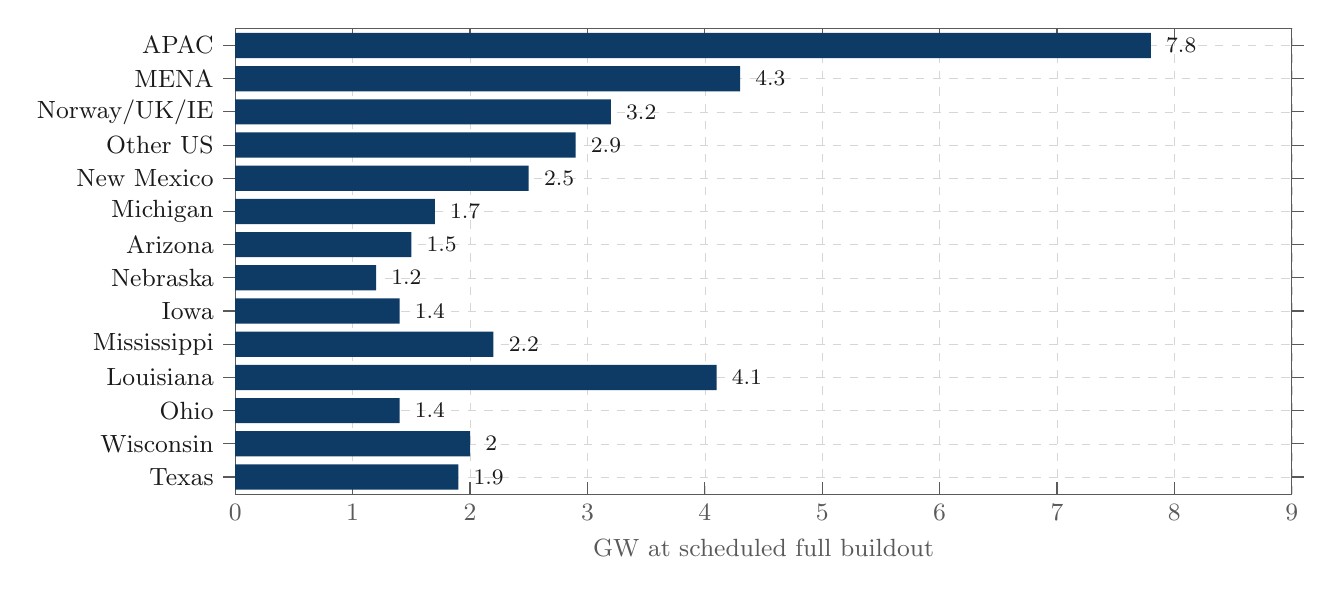
\begin{tikzpicture}
\begin{axis}[
  width=15cm, height=7.5cm,
  xbar,
  bar width=0.32cm,
  enlarge y limits=0.04,
  symbolic y coords={APAC,MENA,NorwayUKIE,OtherUS,NewMexico,Michigan,Arizona,Nebraska,Iowa,Mississippi,Louisiana,Ohio,Wisconsin,Texas},
  yticklabels={APAC,MENA,Norway/UK/IE,Other US,New Mexico,Michigan,Arizona,Nebraska,Iowa,Mississippi,Louisiana,Ohio,Wisconsin,Texas},
  ytick=data,
  xlabel={GW at scheduled full buildout},
  xlabel style={font=\small,color=softGrey},
  yticklabel style={font=\small,color=inkBlack},
  xticklabel style={font=\small,color=softGrey},
  xmin=0, xmax=9,
  nodes near coords,
  nodes near coords style={font=\footnotesize,color=inkBlack,anchor=west,xshift=2pt},
  nodes near coords align={horizontal},
  axis line style={softGrey,thin},
  tick style={softGrey,thin},
  grid=major, grid style={paleGrey,dashed,very thin},
]
\addplot[fill=chartA,draw=none] coordinates {
  (7.8,Texas) (4.3,Wisconsin) (3.2,Ohio) (2.9,Louisiana)
  (2.5,Mississippi) (1.7,Iowa) (1.5,Nebraska) (1.2,Arizona)
  (1.4,Michigan) (2.2,NewMexico) (4.1,OtherUS)
  (1.4,NorwayUKIE) (2.0,MENA) (1.9,APAC)
};
\end{axis}
\end{tikzpicture}
\caption{Scheduled full-buildout capacity by US state and non-US region. Geographic aggregation of Epoch-evidenced sites plus sited commitments from the overlay. Texas alone represents approximately \textbf{one-sixth of the global 2030 pipeline}, driven by ERCOT's faster interconnection timelines and lower marginal power costs relative to grid-constrained alternatives.\protect\footnotemark}
\end{figure}
\footnotetext{Site-level state assignments from Epoch AI address fields; regional aggregation by author. Non-US regions consolidated at continental granularity because of smaller site counts: Norway/UK/Ireland includes Microsoft Narvik, Loughton, Dublin, and Nscale-CoreWeave UK sites; MENA includes Saudi (HUMAIN), UAE (G42/Khazna, Stargate UAE); APAC includes India (Reliance Jamnagar), Singapore, and Australia.}

\subsection{Power, not permits, is the binding constraint}

Publicly disclosed site events routinely show land purchase and construction permits preceding grid interconnection by 18--30 months. The ERCOT queue contains roughly 150 GW of large-load requests against approximately 5 GW per year of deliverable new transmission capacity; PJM's queue is comparably congested.\footnote{ERCOT, \emph{Large Load Interconnection Report}, January 2026. \url{https://www.ercot.com/}; PJM Interconnection, \emph{2024 Regional Transmission Expansion Plan}, Window 3.} The constraint is increasingly addressed via behind-the-meter generation, particularly natural-gas turbines co-located with campuses (Oracle Stargate Abilene; xAI Colossus 2, Memphis) and nuclear power purchase agreements (Microsoft's contract with Constellation Energy for Three Mile Island Unit 1 output;\footnote{Microsoft and Constellation Energy, \emph{Constellation and Microsoft sign agreement to launch Crane Clean Energy Center}, September 20, 2024, \url{https://www.constellationenergy.com/newsroom/2024/crane-clean-energy-center.html}.} Amazon's partnership with Talen Energy at the Susquehanna nuclear facility\footnote{Talen Energy, \emph{Talen Energy reaches agreement with Amazon Web Services for 1{,}920~MW data campus}, March 4, 2024. \url{https://www.talenenergy.com/}}). Roughly one-third of disclosed site-level power-sourcing discussion since 2024 references behind-the-meter generation as the primary path to grid independence.

% ============================================================================
\section{The operators: who owns the horizon}
% ============================================================================

Ten counterparties effectively control the Western 2030 horizon. Their balance sheets, revenue models, and financing structures differ sharply. Understanding who is paying for what requires distinguishing three operator archetypes: \textbf{hyperscalers} (Microsoft, Amazon, Google, Meta), building for both internal consumption and third-party cloud; \textbf{frontier labs} (OpenAI, Anthropic, xAI), consuming compute through long-dated commitments to hyperscalers and neoclouds; and \textbf{merchant neoclouds} (CoreWeave, Nebius, Crusoe, Lambda, Applied Digital, Fluidstack, Nscale, Voltage Park, Together AI), operating dedicated AI capacity under long-dated take-or-pay contracts with hyperscalers and labs.

\subsection{Microsoft: the largest operational AI compute footprint}

Microsoft operates approximately \textbf{1.25 GW} of AI-relevant capacity today, concentrated in the Fairwater programme and associated international sites.\footnote{Epoch AI \emph{Frontier Data Centers}, Microsoft Fairwater Wisconsin (555~MW current), Atlanta (433~MW), Goodyear (263~MW), totalling 1{,}251~MW across Epoch-tracked Microsoft sites.} Announced buildout through 2030 totals approximately \textbf{5 GW of additional Microsoft-owned capacity}, concentrated at Fairwater Wisconsin (targeting 3.3~GW), Fairwater Mississippi, Fairwater Atlanta, Fairwater Cheyenne, Fairwater Narvik (Norway), Fairwater Loughton (United Kingdom), and Fairwater Dublin.\footnote{Microsoft, \emph{Inside the world's most powerful AI datacenter}, September 18, 2025, \url{https://news.microsoft.com/source/features/ai/inside-the-worlds-most-powerful-ai-datacenter/}; Microsoft press releases on Atlanta expansion (November 12, 2025) and international Fairwater siting (September 18, 2025).} Financing is from Microsoft's own operating cash flow --- fiscal-year-2026 capital expenditure guidance exceeds \$100~billion, with the AI share concentrated in the data-centre build.\footnote{Microsoft Corporation, \emph{Q2 FY2026 earnings prepared remarks}, January 28, 2026, Satya Nadella: ``We expect capital expenditures to increase on a sequential basis from the \$19.4 billion reported this quarter ... driven by cloud and AI demand''; Amy Hood: ``FY2026 capital expenditures are expected to be meaningfully above fiscal year 2025.'' Microsoft FY2025 capex totalled \$88.2 billion; author's extrapolation of FY2026 to the \$110--120 billion range.}

Microsoft also serves as the \textbf{exclusive cloud provider to OpenAI for first-party API workloads until at least January 2030}, a relationship restructured in the October 2025 Microsoft--OpenAI financial and operational agreement.\footnote{Microsoft Corporation and OpenAI, \emph{Restructured commercial agreement}, October 28, 2025, as disclosed in Microsoft's 10-Q for Q1 FY2026. \url{https://www.microsoft.com/en-us/investor}} This makes a substantial fraction of the Stargate consumption attributable to Microsoft's Azure franchise rather than OpenAI's direct procurement.

\subsection{Amazon and Anthropic: Project Rainier and the April 2026 expansion}

Amazon operates approximately \textbf{1.43 GW} of AI-relevant capacity today, of which roughly \textbf{1.09 GW is dedicated to Anthropic} via the New Carlisle (Indiana) campus, built in AWS's direct-air-cooled modular architecture.\footnote{Epoch AI, site entry ``Anthropic-Amazon New Carlisle'': ``It is similar to other Amazon locations forgoing most external cooling infrastructure in favor of direct air based cooling.'' Current power: 1{,}092~MW. Attribution: Amazon \#confident, Anthropic \#confident.} Additional AWS AI sites at Madison (Indiana, 341~MW current) and Ridgeland (Mississippi, growing into 1.3~GW) round out the Amazon-AI footprint.\footnote{Epoch AI, site entries ``Amazon Madison'' and ``Amazon Ridgeland''. Ridgeland current: approximately 300~MW; full buildout: 1{,}008~MW by 2028.}

On April 20, 2026, Anthropic and Amazon announced an expansion committing \textbf{up to 5 additional gigawatts of new capacity on AWS}, with the first gigawatt scheduled for end-of-year 2026 and the balance delivered through 2030.\footnote{Anthropic and Amazon, \emph{Anthropic and Amazon expand collaboration for up to 5 gigawatts of new compute}, April 20, 2026. \url{https://www.anthropic.com/news/anthropic-amazon-compute}. Verbatim: ``up to 5 gigawatts (GW) of new capacity'' and ``more than \$100 billion over the next ten years on AWS technologies''.} The expansion is \textbf{explicitly anchored on AWS Trainium silicon}: Anthropic's April 7, 2026 engineering blog confirms that Project Rainier's primary training compute is AWS Trainium~2, and that Trainium~3 delivers roughly a three-to-four-fold per-chip throughput uplift.\footnote{Anthropic, \emph{Expanding our use of Google Cloud TPUs}, April 7, 2026. \url{https://www.anthropic.com/news/expanding-our-use-of-google-cloud-tpus}. Quote: Anthropic describes ``a diversified compute strategy'' with AWS Trainium and Google TPU as primary training platforms.} This means Anthropic's largest training cluster worldwide --- already larger than any individual OpenAI Stargate site at present --- runs on \textbf{non-NVIDIA silicon}. The commercial reality of chip diversification at the frontier lab tier is therefore already considerably more advanced than is commonly portrayed.

\subsection{OpenAI: Stargate and triple-vendor chip procurement}

OpenAI consumes compute via three primary channels: Microsoft Azure (the original exclusive cloud relationship, continued through January 2030 for first-party API workloads), Oracle Cloud Infrastructure (the eight-site Stargate programme), and direct NVIDIA / AMD / Broadcom silicon commitments that deploy into the above shells.

The \textbf{Stargate programme totals eight named US sites with an aggregate full-buildout capacity of approximately 10.6 GW}, anchored on Oracle as operator and the SoftBank-MGX-Oracle ``Stargate LP'' capital structure announced January 21, 2025.\footnote{OpenAI, \emph{Announcing the Stargate Project}, January 21, 2025. \url{https://openai.com/index/announcing-the-stargate-project}. The original commitment language: ``\$500 billion over the next four years'' with ``\$100 billion deploying immediately''.} The September 24, 2025 expansion added five new sites (Shackelford, Lordsburg, Milam, Doña Ana, and one additional undisclosed location), collectively specified as ``nearly 7 gigawatts''.\footnote{OpenAI, \emph{Five new Stargate sites}, September 24, 2025. \url{https://openai.com/index/five-new-stargate-sites/}}

OpenAI is the \textbf{only frontier operator with material, disclosed commitments to three chip vendors simultaneously}: a 10-gigawatt NVIDIA letter-of-intent announced September 22, 2025, a 6-gigawatt AMD Instinct commitment announced October 6, 2025, and a 10-gigawatt custom-ASIC commitment with Broadcom announced October 13, 2025.\footnote{NVIDIA Corporation and OpenAI, \emph{NVIDIA and OpenAI announce partnership of unprecedented scale}, September 22, 2025, \url{https://nvidianews.nvidia.com/news/nvidia-openai-partnership}; Advanced Micro Devices and OpenAI, \emph{AMD and OpenAI announce strategic partnership for 6 gigawatts of AMD Instinct}, October 6, 2025, \url{https://ir.amd.com/news-events/press-releases/detail/1276/amd-and-openai-announce-strategic-partnership}; Broadcom Inc.\ and OpenAI, October 13, 2025. Note: the 26~GW aggregate across these three LOIs deploys into Stargate and Microsoft Azure shells already counted in the physical-site census.} These three commitments aggregate to 26 GW of chips, but \textbf{do not represent additional physical capacity} --- they deploy into Stargate and Azure shells already counted in the site-level census.

\subsection{Meta: Hyperion, Prometheus, and the Nebius partnership}

Meta operates approximately \textbf{730 MW} of AI capacity today across the Prometheus and Temple sites, with the Hyperion superintelligence campus in Richland Parish, Louisiana (MISO-South via Entergy Louisiana) scheduled to reach \textbf{approximately 2.3 GW by 2028}.\footnote{Meta Platforms, \emph{Introducing Hyperion: Meta AI superintelligence data center}, July 14, 2025. \url{https://about.fb.com/news/2025/07/introducing-hyperion-meta-ai-superintelligence-data-center/}. Meta's newsroom language: ``over 2 gigawatts''. Epoch AI tracks full buildout at 2{,}262~MW.} Mark Zuckerberg's Q2~2025 earnings remarks, subsequently reiterated on Q3 and Q4, describe a \textbf{stretch target of 5 gigawatts} for the Hyperion complex ``over the next several years,'' representing an additional ~2.7 GW beyond the newsroom-committed base.\footnote{Meta Platforms, Q2~2025 earnings call, July 30, 2025, Mark Zuckerberg: ``We're building multiple multi-gigawatt data centers ... Hyperion is expected to scale up to 5 gigawatts over several years.'' \url{https://investor.fb.com/} Meta earnings transcripts.}

On March 16, 2026, Meta signed a \textbf{\$27 billion five-year take-or-pay agreement with Nebius for dedicated capacity at Nebius's Vineland, New Jersey campus},\footnote{Nebius Group N.V., \emph{Nebius signs \$27 billion agreement with Meta}, March 16, 2026. \url{https://group.nebius.com/news-and-updates/nebius-signs-27-billion-agreement-with-meta}. Vineland NJ site disclosed in Nebius Q4~FY2025 shareholder letter, February 20, 2026.} making Meta the first Big Tech operator to source material capacity from a merchant neocloud at this scale. Meta also began disclosing \textbf{second-generation MTIA (Meta Training and Inference Accelerator)} deployments in 2025 earnings commentary, indicating that Hyperion's outer-phase silicon will combine NVIDIA Blackwell/Rubin with Meta's own inference ASIC fleet.\footnote{Meta Platforms, Q4~2025 earnings call, January 28, 2026. Discussion of MTIA v2 in-production deployment and MTIA v3 roadmap.}

\subsection{Google: TPU supply to Anthropic and the Gemini internal fleet}

Google operates approximately \textbf{956 MW} of AI-relevant capacity across five Epoch-tracked TPU sites (Council Bluffs East and West, Omaha, New Albany, Cedar Rapids), with several additional non-AI-dominant Google Cloud sites not separately broken out.\footnote{Epoch AI \emph{Frontier Data Centers}, Google sites. Council Bluffs (combined): 597~MW current; Omaha: 189~MW; New Albany: 407~MW; Cedar Rapids: 105~MW.}

The most commercially consequential Google commitment on the horizon is the \textbf{Anthropic TPU partnership}: up to one million TPU chips, ``well over a gigawatt of capacity coming online in 2026,'' and --- per Anthropic's April 7, 2026 expansion announcement and Broadcom's Q1 FY2026 earnings call --- an additional \textbf{3.5 gigawatts of TPU capacity starting in 2027}.\footnote{Anthropic and Google Cloud, \emph{Expanding our partnership: up to one million TPU chips}, October 23, 2025, \url{https://www.anthropic.com/news/anthropic-google-cloud}. Expansion: Anthropic, \emph{Expanding our use of Google Cloud TPUs}, April 7, 2026, \url{https://www.anthropic.com/news/expanding-our-use-of-google-cloud-tpus}. Broadcom confirmation: Broadcom Inc., Q1~FY2026 earnings call, March 6, 2026, Hock Tan: 3.5 GW XPU commitment from a named customer. Anthropic subsequently confirmed counterparty identity in the April 7 blog.} On April 22, 2026, Google Cloud unveiled the \textbf{eighth-generation TPU} (TPU v8 in two variants: 8t for training, 8i for inference) alongside an expanded partnership with NVIDIA for A5X Vera Rubin instances on Google Cloud.\footnote{Google Cloud, \emph{Google Cloud AI infrastructure at NVIDIA GTC 2026}, April 22, 2026, \url{https://cloud.google.com/blog/products/compute/google-cloud-ai-infrastructure-at-nvidia-gtc-2026}; NVIDIA Corporation, \emph{NVIDIA and Google Cloud expand partnership to scale AI development}, April 22, 2026.}

\subsection{xAI: the fastest-built AI campus on record}

xAI operates approximately \textbf{425 MW} of AI-relevant capacity at the original Memphis Colossus campus (MISO via Memphis Light, Gas \& Water). The planned Colossus~2 site, also in Memphis and disclosed July 31, 2025, is scheduled for 2027 completion targeting \textbf{approximately 2 GW of IT-relevant capacity} (approximately 2.6~GW facility at PUE~1.30).\footnote{xAI, \emph{Colossus~2 announcement}, July 31, 2025. \url{https://x.ai/news/colossus-2}. Epoch AI tracks Colossus~2 at 1{,}494~MW full buildout.} In November 2025, xAI announced a joint-venture with HUMAIN (Saudi Arabia's Public Investment Fund AI subsidiary) for a \textbf{500~MW+ sovereign campus with ``18{,}000 NVIDIA GB300 GPUs in first cluster''}.\footnote{Reuters, \emph{xAI and HUMAIN announce 500~MW Saudi Arabia partnership}, November 12, 2025. First cluster: ``18{,}000 NVIDIA GB300 GPUs'' per joint announcement.}

\subsection{The merchant neoclouds: 9.4 GW of take-or-pay contracted capacity}

The frontier neocloud segment has transitioned from a boutique GPU-hosting business in 2023 to a category materially contracted to investment-grade counterparties in 2026. CoreWeave disclosed \textbf{\$60.7 billion in remaining performance obligations (RPO)} at fiscal-year-2025 close, anchored on 15-year take-or-pay agreements with Microsoft and OpenAI.\footnote{CoreWeave, Inc., \emph{FY2025 Form 10-K}, filed February 26, 2026. ASC~606 remaining performance obligation: \$60.7 billion; total revenue backlog: \$66.8 billion. \url{https://www.sec.gov/cgi-bin/browse-edgar}} Nebius disclosed aggregate contracted backlog in the \textbf{\$44.4--46.4 billion range} at FY2025 close, principally the \$27 billion Meta agreement and an approximately \$19.4 billion Microsoft agreement announced in 2025.\footnote{Nebius Group, Q4 FY2025 shareholder letter filed on 6-K, February 20, 2026. FY2025 20-F filing scheduled for April 30, 2026. Microsoft contract reported in Reuters, September 2025, not independently disclosed by Nebius beyond financial-aggregate form.} Applied Digital raised \textbf{\$2.15 billion of 6.75\% senior secured notes due 2031} in March 2026 to fund the Ellendale campus under a CoreWeave lease; the notes are rated A3 by Moody's on a special-purpose-vehicle credit basis.\footnote{Applied Digital Corporation, Form 8-K filed March 30, 2026, disclosing \$2.15~billion aggregate principal senior secured notes; Moody's Investors Service, rating action A3, March 30, 2026. Applied Digital Q3 FY2026 10-Q filed April 8, 2026.}

The aggregate neocloud-ex-Epoch operational and contracted capacity is approximately \textbf{9.4 GW} through 2030, making the neocloud segment --- despite its sub-investment-grade operator credit --- a larger contributor to the 2030 horizon than any single hyperscaler other than Microsoft and the Anthropic-dedicated portion of Amazon.

% ============================================================================
\section{The silicon: NVIDIA, Trainium, TPU, AMD, Broadcom, MTIA}
% ============================================================================

The silicon landscape is \textbf{more diversified at the frontier lab tier than at the hyperscaler tier}. Measured by deployed and contracted compute through 2030, NVIDIA retains approximately \textbf{two-thirds share} of the Western horizon's chip dollars. But at the individual-frontier-lab level, three of the four leading Western labs --- Anthropic, Google (DeepMind), and Meta --- now source a substantial fraction of their training compute from non-NVIDIA silicon.

\subsection{Four generations of frontier chips in four years}

The chip-generation cadence is the single most important forward parameter in the build-out. Each new generation approximately doubles the 8-bit floating-point throughput per watt, which means site-level compute roughly doubles every two years even on a constant physical-GW footprint.

\begin{figure}[h]
\centering
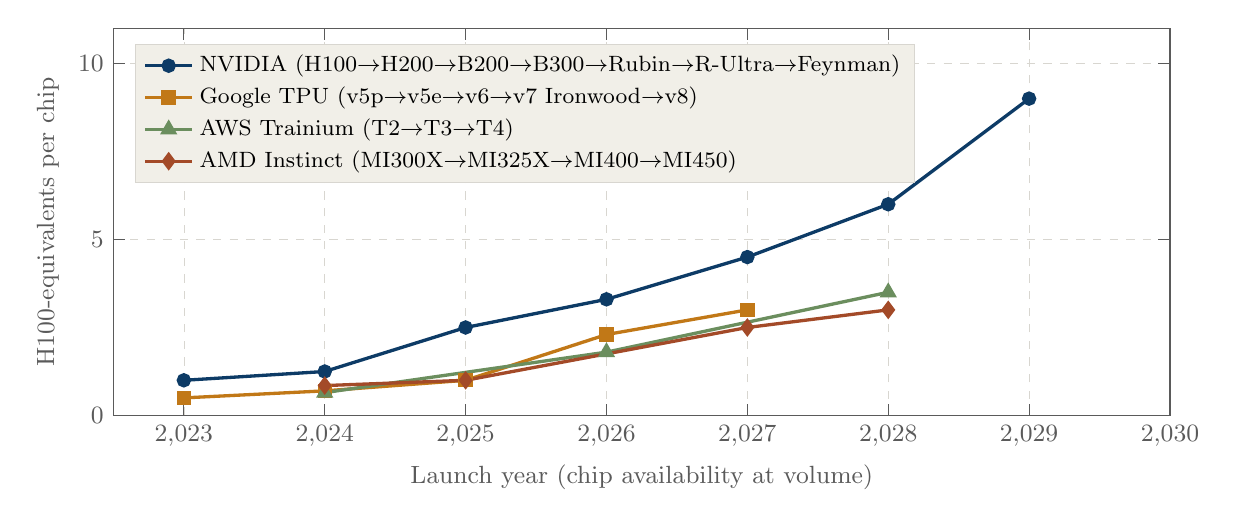
\begin{tikzpicture}
\begin{axis}[
  width=15cm, height=6.5cm,
  xlabel={Launch year (chip availability at volume)},
  ylabel={H100-equivalents per chip},
  xlabel style={font=\small,color=softGrey},
  ylabel style={font=\small,color=softGrey},
  xmin=2022.5, xmax=2030,
  ymin=0, ymax=11,
  xtick={2023,2024,2025,2026,2027,2028,2029,2030},
  xticklabel style={font=\small,color=softGrey},
  yticklabel style={font=\small,color=softGrey},
  axis line style={softGrey,thin},
  tick style={softGrey,thin},
  grid=major, grid style={paleGrey,dashed,very thin},
  legend style={at={(0.02,0.96)},anchor=north west,font=\footnotesize,draw=paleGrey,fill=lightCream},
  legend cell align={left},
]
% NVIDIA curve
\addplot[color=chartA,line width=1.2pt,mark=*,mark size=2pt] coordinates {
  (2023, 1.0) (2024, 1.25) (2025, 2.5) (2026, 3.3) (2027, 4.5) (2028, 6.0) (2029, 9.0)
};
\addlegendentry{NVIDIA (H100$\rightarrow$H200$\rightarrow$B200$\rightarrow$B300$\rightarrow$Rubin$\rightarrow$R-Ultra$\rightarrow$Feynman)}
% Google TPU curve
\addplot[color=chartB,line width=1.2pt,mark=square*,mark size=2pt] coordinates {
  (2023, 0.5) (2024, 0.7) (2025, 1.0) (2026, 2.3) (2027, 3.0)
};
\addlegendentry{Google TPU (v5p$\rightarrow$v5e$\rightarrow$v6$\rightarrow$v7 Ironwood$\rightarrow$v8)}
% AWS Trainium curve
\addplot[color=chartC,line width=1.2pt,mark=triangle*,mark size=2.4pt] coordinates {
  (2024, 0.65) (2026, 1.8) (2028, 3.5)
};
\addlegendentry{AWS Trainium (T2$\rightarrow$T3$\rightarrow$T4)}
% AMD Instinct curve
\addplot[color=chartD,line width=1.2pt,mark=diamond*,mark size=2.4pt] coordinates {
  (2024, 0.85) (2025, 1.0) (2027, 2.5) (2028, 3.0)
};
\addlegendentry{AMD Instinct (MI300X$\rightarrow$MI325X$\rightarrow$MI400$\rightarrow$MI450)}
\end{axis}
\end{tikzpicture}
\caption{Per-chip H100-equivalents by chip family and launch year. NVIDIA maintains per-chip throughput leadership, but AWS Trainium~3 and Google TPU v7 Ironwood both materially close the gap in 2026--2027. The 2028--2029 generation (NVIDIA Feynman, Trainium~4, TPU v9, AMD MI450) is projected based on published roadmap disclosures; actual per-chip figures are subject to taping-out and yield at the respective foundry partners.\protect\footnotemark}
\end{figure}
\footnotetext{Per-chip H100e values computed from published 8-bit OP/s throughput disclosures: NVIDIA GTC keynotes 2023--2026; Google Cloud Next 2025--2026 TPU specifications; AWS re:Invent 2023--2025 Trainium disclosures; AMD Advancing AI events 2023--2025. Post-2027 values extrapolated from roadmap announcements and are explicitly projections, not confirmed silicon.}

\subsection{Chip vendor share across the Western horizon}

Aggregating the chip commitments across the hyperscaler, frontier-lab, and neocloud segments for the full 2030 horizon produces a vendor-share distribution that differs markedly from the 2024--2025 marketplace.

\begin{figure}[h]
\centering
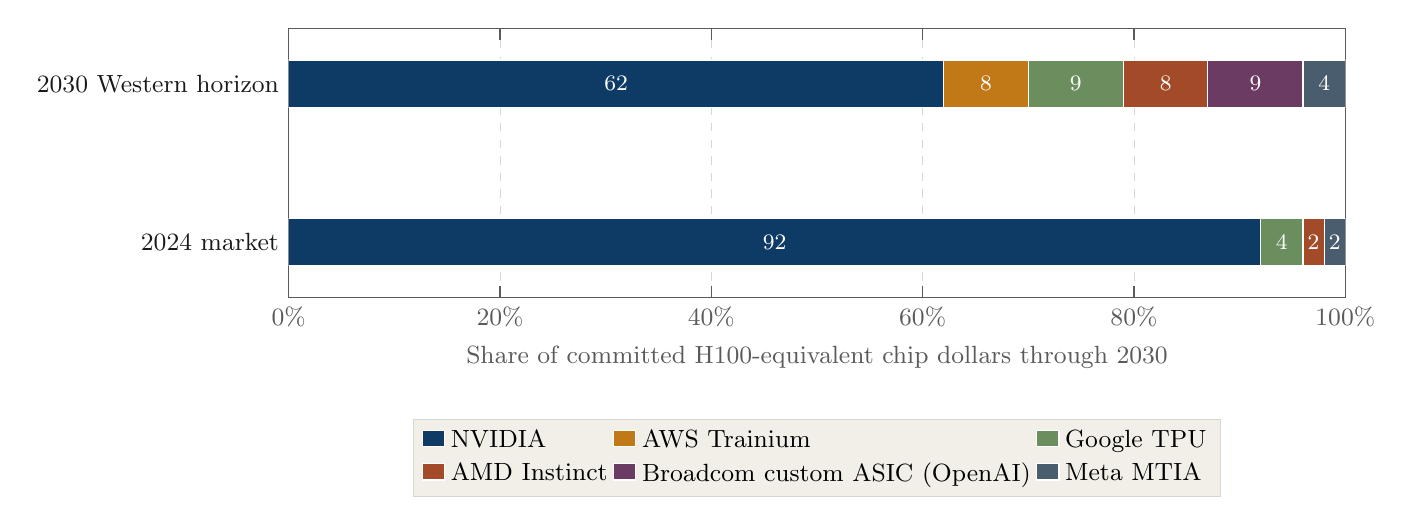
\begin{tikzpicture}
\begin{axis}[
  width=15cm, height=5cm,
  xbar stacked,
  bar width=0.6cm,
  enlarge y limits=0.35,
  symbolic y coords={y2024,y2030},
  ytick=data,
  yticklabels={2024 market,2030 Western horizon},
  xlabel={Share of committed H100-equivalent chip dollars through 2030},
  xlabel style={font=\small,color=softGrey},
  yticklabel style={font=\small,color=inkBlack},
  xticklabel style={font=\small,color=softGrey},
  xmin=0, xmax=100,
  xtick={0,20,40,60,80,100},
  xticklabel={\pgfmathprintnumber{\tick}\%},
  axis line style={softGrey,thin},
  tick style={softGrey,thin},
  grid=major, grid style={paleGrey,dashed,very thin},
  legend style={at={(0.5,-0.45)},anchor=north,font=\small,draw=paleGrey,fill=lightCream,legend columns=3},
  legend cell align={left},
  nodes near coords,
  nodes near coords style={font=\footnotesize,color=white,align=center},
  every node near coord/.append style={/pgf/number format/.cd,fixed,precision=0},
]
\addplot[fill=chartA,draw=white] coordinates {(92,y2024) (62,y2030)};
\addlegendentry{NVIDIA}
\addplot[fill=chartB,draw=white] coordinates {(0,y2024) (8,y2030)};
\addlegendentry{AWS Trainium}
\addplot[fill=chartC,draw=white] coordinates {(4,y2024) (9,y2030)};
\addlegendentry{Google TPU}
\addplot[fill=chartD,draw=white] coordinates {(2,y2024) (8,y2030)};
\addlegendentry{AMD Instinct}
\addplot[fill=chartE,draw=white] coordinates {(0,y2024) (9,y2030)};
\addlegendentry{Broadcom custom ASIC (OpenAI)}
\addplot[fill=chartF,draw=white] coordinates {(2,y2024) (4,y2030)};
\addlegendentry{Meta MTIA}
\end{axis}
\end{tikzpicture}
\caption{Approximate share of committed chip-capital dollars by vendor, 2024 snapshot vs.\ 2030 Western horizon. NVIDIA retains majority share but loses roughly 30 percentage points to the combined AWS+Google+AMD+Broadcom+Meta diversification. Shares estimated from published commitments and roadmap volumes.\protect\footnotemark}
\end{figure}
\footnotetext{Author's aggregation from operator-disclosed chip commitments: Anthropic Project Rainier (Trainium); Anthropic TPU (1M chips + 3.5 GW expansion); OpenAI--NVIDIA (10 GW), OpenAI--AMD (6 GW Instinct), OpenAI--Broadcom (10 GW custom ASIC); Meta MTIA deployment commentary; Microsoft--NVIDIA Fairwater silicon. Individual percentage estimates carry material uncertainty because most commitments are disclosed in GW or chip-count rather than dollar terms; dollar share derived using vendor-specific ASP assumptions.}

\subsection{The commercial reality of Anthropic's silicon}

Anthropic's disclosed silicon posture is worth pausing on because it illustrates the commercial distance between ``NVIDIA-dominant'' as a marketplace observation and ``NVIDIA-exclusive'' as a training decision for a specific lab. Anthropic's largest training cluster today is the Amazon-operated New Carlisle campus, which runs \textbf{AWS Trainium~2} as its primary accelerator.\footnote{Amazon Web Services and Anthropic, \emph{Announcing Project Rainier}, November 13, 2024; Anthropic, \emph{Expanding our use of Google Cloud TPUs}, April 7, 2026, confirming Trainium-backbone training.} Anthropic's second-largest committed training capacity is the Google-operated TPU programme, at \textbf{up to one million TPU chips plus 3.5 GW of TPU v7/v8 capacity from 2027 onward}. Anthropic's NVIDIA deployment --- via Nscale-Fluidstack and Microsoft-Azure --- is material but secondary to both Trainium and TPU on a dollar-weighted basis.

Put differently: the single largest non-NVIDIA training buildout at the global frontier today is happening at Anthropic, on AWS silicon. The ``NVIDIA has won AI'' framing understates how far chip-diversification has already travelled at the lab tier.

\subsection{H100e sensitivity: conservative, base, aggressive silicon uplift}
\label{subsec:h100e-sensitivity}

The paper's headline figure of 78.2M H100-equivalents by 2030 (revised 2026-04-24 from 78.4M) assumes per-family chip-density trajectories drawn from disclosed roadmaps through 2027 and extrapolations of observed per-generation uplift curves for 2028--2030. That extrapolation is load-bearing: small shifts in the 2028--2030 density assumption move the aggregate H100e count by tens of millions.

What H100-equivalents miss. Before presenting the sensitivity range, three caveats: (i) H100e normalizes 8-bit dense FLOP/s but understates gains in sparsity, lower-precision (FP4/FP6) inference, and memory-bandwidth throughput that matter disproportionately for reasoning-dominated workloads; (ii) networking fabric (NVLink/NVSwitch generations, InfiniBand NDR/XDR, AWS EFAv3) contributes 10--30\% of effective-throughput differences between nominally-equivalent chips; (iii) compiler maturity (CUDA vs XLA vs Neuron) and cluster utilization (discussed in \S9) further decouple nameplate H100e from delivered training throughput. Readers should treat H100e as the least-bad available scalar, not a physical-FLOP count.

\begin{table}[h]
\centering
\small
\begin{tabular}{@{}lrr@{}}
\toprule
\textbf{Scenario} & \textbf{2030 Western H100e (M)} & \textbf{Growth vs.\ 2026 Q2} \\
\midrule
Conservative (hold 2026 density flat) & 60.0 & 12.7$\times$ \\
Base (disclosed roadmaps + observed curves) & 78.2 & 18.6$\times$ \\
Aggressive (straight-line Epoch per-family curve) & 110.0 & 23.2$\times$ \\
\bottomrule
\end{tabular}
\caption{H100-equivalent count in the 2030 Western horizon under three silicon-uplift scenarios. The base case is the figure referenced elsewhere in this paper. Conservative holds per-family H100e/MW flat at 2026 levels (a world where no new chip generation after Blackwell-Ultra meaningfully ships). Aggressive extrapolates Epoch AI's observed per-family H100e/MW curve (NVIDIA has averaged ~2$\times$ per-generation-MW uplift 2022--2026; TPU ~1.7$\times$; Trainium ~2.2$\times$).}
\end{table}

Per-family disclosure status underlying the base case: NVIDIA H100/H200/B200/B300 are disclosed via GTC keynotes and datasheet material; Rubin is roadmap-only through 2027 and extrapolated 2028--2030. Google TPU v5p/v5e/v6/v7~Ironwood/v8 are disclosed through 2026; TPU v9 is inferred. AWS Trainium~2 is disclosed; Trainium~3 is roadmap-disclosed at re:Invent 2025; Trainium~4 is extrapolated. AMD MI300X/MI325X are disclosed; MI400 is roadmap-disclosed; MI450 is inferred. Broadcom custom ASIC (Anthropic XPU, OpenAI XPU, Meta MTIA): disclosed at GW-commitment level, not chip-count or per-chip-throughput level; the silicon-layer contribution from Broadcom programs is the single largest source of aggressive-case upside (and the largest unknown).

The $\pm$30\% uncertainty band around the 78.2M H100e base reading is not precision-inflation: it reflects honest extrapolation risk across six chip families, three foundries (TSMC, Samsung, Intel-foundry), and five compressed cycles of 2-year generational cadence. Anyone forecasting a single H100e number for 2030 without a sensitivity band is overconfident.

% ============================================================================
\section{The \$1.5 trillion question: where the money comes from}
% ============================================================================

The 51.9~GW facility Western horizon (50.6~GW IT-load bridge) carries an estimated \textbf{capital envelope of \$1.2--1.5 trillion between 2026 and 2030} (what must be spent to build it). A separate approximately \textbf{\$550~billion of contracted remaining performance obligations (RPO)} underwrites but does not constitute this capex --- see \S\ref{subsec:financing-bridge}. The capex envelope has four distinct funding channels, each with different balance-sheet exposure, revenue backing, and credit characteristics.

\subsection{Bucket 1: hyperscaler operating cash flow (actual spend and guided)}

\textbf{Four conceptually distinct capital questions.} Before listing the buckets, it is worth naming the confusion this section exists to avoid. ``Who pays'' has four orthogonal answers in the AI build-out: (i) \textbf{capex actually spent or guided} --- the hyperscaler 10-K capex line, which is real money flowing in 2025--2026; (ii) \textbf{capex still required} --- the residual between total build cost and actual-plus-guided, which must be financed from 2027 onward; (iii) \textbf{contracted RPO} --- revenue commitments from labs to infrastructure providers that \emph{underwrite} capex without being capex themselves; and (iv) \textbf{financing source} --- corporate debt, SPV debt, sovereign equity, public-market equity, each of which funds capex through different balance sheets. The Oracle--OpenAI \$300B commitment is a (iii); Microsoft's \$88B FY25 capex is a (i); Applied Digital's \$2.15B senior secured notes are a (iv). These are not substitutes and must not be summed.

The four large US hyperscalers (Microsoft, Amazon, Google, Meta) collectively guided capital expenditures of approximately \textbf{\$400 billion in calendar 2025} and approximately \textbf{\$500 billion in calendar 2026}, with the AI-data-centre share rising from roughly 60\% to 75\% of total capex across the two years.\footnote{Microsoft: FY2025 capex \$88.2B (10-K filed July 31, 2025), FY2026 guided ``meaningfully above'' (Q2 FY2026 earnings, January 28, 2026). Amazon: Andy Jassy Q4 2025 commentary, February 5, 2026: ``We expect 2026 capital expenditures to be notably higher than 2025's \$125B''; \url{https://ir.aboutamazon.com/}. Alphabet: Ruth Porat Q4 2025 commentary, February 4, 2026: ``2026 capital expenditures will be approximately \$85 billion''. Meta: Susan Li Q4 2025 commentary, January 28, 2026: ``2026 total expenses of \$175--\$200B ... capital expenditures of \$80--\$95B''. Sources: respective Q4 2025 earnings calls and subsequent 10-K filings.} Across two years, the four-hyperscaler aggregate is roughly \textbf{\$550--650 billion of AI-attributable capex}, which alone funds more than a third of the 2030 horizon.

\begin{figure}[h]
\centering
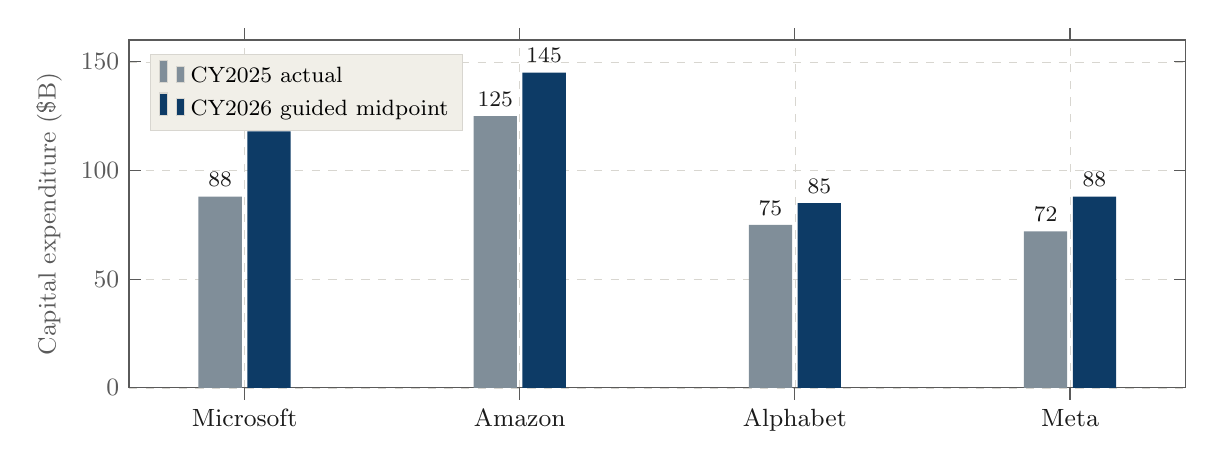
\begin{tikzpicture}
\begin{axis}[
  width=15cm, height=6cm,
  ybar,
  bar width=0.55cm,
  enlarge x limits=0.14,
  symbolic x coords={Microsoft, Amazon, Alphabet, Meta},
  xtick=data,
  xticklabel style={font=\small,color=inkBlack},
  ylabel={Capital expenditure (\$B)},
  ylabel style={font=\small,color=softGrey},
  yticklabel style={font=\small,color=softGrey},
  ymin=0, ymax=160,
  axis line style={softGrey,thin},
  tick style={softGrey,thin},
  grid=major, grid style={paleGrey,dashed,very thin},
  legend style={at={(0.02,0.96)},anchor=north west,font=\footnotesize,draw=paleGrey,fill=lightCream,legend columns=1},
  legend cell align={left},
  nodes near coords,
  nodes near coords style={font=\footnotesize,color=inkBlack,anchor=south},
]
\addplot[fill=chartF!70,draw=none] coordinates {(Microsoft, 88) (Amazon, 125) (Alphabet, 75) (Meta, 72)};
\addlegendentry{CY2025 actual}
\addplot[fill=chartA,draw=none] coordinates {(Microsoft, 118) (Amazon, 145) (Alphabet, 85) (Meta, 88)};
\addlegendentry{CY2026 guided midpoint}
\end{axis}
\end{tikzpicture}
\caption{Big-Four hyperscaler capital expenditure, calendar-year 2025 actuals and calendar-year 2026 guidance midpoints. The AI-data-centre share of capex has risen from approximately 60\% in CY2024 to roughly 75\% in CY2026 guidance, with the residual allocated to non-AI cloud infrastructure, office real estate, and maintenance.\protect\footnotemark}
\end{figure}
\footnotetext{CY2025 actuals: Microsoft FY2025 10-K; Amazon Q4 2025 earnings (FY = CY); Alphabet Q4 2025 earnings (FY = CY); Meta Q4 2025 earnings (FY = CY). CY2026 guidance: from respective Q4 2025 earnings calls and subsequent 10-K filings as of April 2026. Microsoft FY2026 figures adjusted to a calendar-year basis by linear interpolation across the June-ending fiscal year.}

\subsection{Bucket 2: contracted RPO (revenue obligations, not capex)}
\label{subsec:rpo-bucket}

The single largest contracted-revenue commitment in the history of enterprise cloud is the Oracle--OpenAI agreement, disclosed in Oracle's Q1 FY2026 10-Q as a \textbf{\$300 billion five-year take-or-pay commitment from OpenAI} beginning in 2027.\footnote{Oracle Corporation, Form 10-Q for Q1 FY2026, filed September 10, 2025. Oracle disclosed ``a \$300 billion, five-year purchase commitment'' from a named customer (subsequently confirmed as OpenAI in Oracle's Q2 FY2026 earnings call, December 9, 2025, Larry Ellison). \url{https://www.sec.gov/cgi-bin/browse-edgar}} The Oracle--OpenAI commitment is the single largest capex-underwriting contract signed in the industry. \textbf{It is a revenue obligation from OpenAI to Oracle, not a capex channel:} the \$300~B appears in Oracle's income statement as contracted future revenue, and separately enables Oracle to finance Stargate shell construction via a combination of corporate debt, SPV debt, and retained earnings. In this paper it is counted in the RPO bucket (\S\ref{subsec:financing-bridge}), not in the capex bucket.

Additional take-or-pay commitments include: \textbf{Anthropic--Amazon at ``more than \$100 billion over ten years''} (April 20, 2026 announcement);\footnote{Anthropic and Amazon, April 20, 2026. Amazon's 10-K will disclose aggregate RPO from this agreement in Q2 FY2026 filings.} \textbf{Anthropic--Google TPU estimated at \$52--60 billion} based on the ``up to one million chips'' language and published TPU v7 pricing;\footnote{Anthropic, \emph{Expanding our use of Google Cloud TPUs}, April 7, 2026; Alphabet Q1 FY2026 10-Q, filed April 24, 2026 (expected), for aggregate RPO disclosure. Industry estimate: approximately \$52--60 billion.} \textbf{CoreWeave--Microsoft and CoreWeave--OpenAI at a combined approximately \$50 billion in 15-year take-or-pay}, already reflected in CoreWeave's \$60.7 billion FY2025 RPO.\footnote{CoreWeave, Inc.\ FY2025 10-K, Note~12 (Contract Balances), disclosing RPO of \$60.7~billion. Microsoft contract announced 2022; OpenAI contract announced March 2025.} \textbf{Nebius--Meta at \$27 billion} (March 16, 2026);\footnote{Nebius Group, \emph{Nebius signs \$27 billion agreement with Meta}, March 16, 2026.} and \textbf{Nebius--Microsoft at approximately \$19.4 billion}.\footnote{Reuters, September 2025, reporting disclosed Nebius--Microsoft contract value. Nebius aggregate RPO disclosed in Q4 FY2025 shareholder letter; individual counterparty values not separately disclosed by Nebius.}

\subsection{Bucket 3: neocloud debt (financing source, not capex)}

The merchant-neocloud segment has become a significant debt issuer over 2024--2026, supported by the investment-grade counterparty credit behind the take-or-pay revenue. Applied Digital's \textbf{\$2.15 billion of 6.75\% senior secured notes due 2031}, issued March 2026 at an A3 Moody's rating on the SPV pledged to the CoreWeave Ellendale lease, exemplifies the model.\footnote{Applied Digital Corporation, Form 8-K filed March 30, 2026; Moody's Investors Service rating action, March 30, 2026.} CoreWeave has issued multiple tranches of delayed-draw term loans secured by its GPU fleet, collectively in the \$15--20 billion range, against the Microsoft/OpenAI 15-year RPO backlog.\footnote{CoreWeave FY2025 10-K, Note~7 (Debt). Credit agreements with Blackstone, Magnetar, and various other private-credit lenders.}

\subsection{Bucket 4: sovereign wealth (financing source)}

Abu Dhabi's MGX, Saudi Arabia's Public Investment Fund (through HUMAIN), Reliance Industries (India), and the UK government's Department for Science, Innovation and Technology (DSIT) together contribute an estimated \textbf{\$150--250 billion of state-backed capital} to the global AI buildout 2026--2030.\footnote{MGX is a 2025-formed Abu Dhabi sovereign AI investment vehicle, partnered in the OpenAI Stargate consortium (\$100~B initial tranche, \$500~B ten-year vehicle per January 21, 2025 OpenAI release). HUMAIN is the Saudi Public Investment Fund's AI subsidiary (incorporated March 2025), deploying the \$10 billion AMD joint venture and the xAI sovereign 500~MW campus. UK DSIT's AI Opportunities Action Plan commits approximately £5 billion (announced January 13, 2025, \url{https://www.gov.uk/government/publications/ai-opportunities-action-plan}). Reliance Industries: Mukesh Ambani's 47th AGM address, August 29, 2024, references ``gigawatt-scale'' capacity at Jamnagar.} Because sovereign-AI programmes carry structurally different revenue models and grid-connection dynamics, they are described separately in Section~8.

\subsection{Capex bridge: what the money pays for}
\label{subsec:capex-bridge}

The \$1.2--1.5 trillion capital envelope decomposes across five distinct capex categories. Understanding the split matters because the supply-chain, permitting, and execution risk differs sharply across them: physical shells have a 24--36 month lead time, accelerators are constrained by wafer-start and HBM capacity, power and cooling infrastructure hinges on utility and substation delivery, networking scales more linearly with demand, and land/permitting is one-time.

\begin{table}[h]
\centering
\small
\begin{tabular}{@{}lrrl@{}}
\toprule
\textbf{Capex category} & \textbf{\$B (low)} & \textbf{\$B (high)} & \textbf{Binding constraint} \\
\midrule
Accelerators (GPU/TPU/ASIC) & 650 & 850 & TSMC CoWoS + HBM \\
Physical shell (building + fit-out) & 180 & 230 & 24--36 mo build cycle \\
Power + cooling + substation & 200 & 260 & Utility/ISO queue \\
Networking (intra + inter-DC) & 100 & 130 & ASIC wafer starts \\
Land + permitting + transmission & 70 & 90 & Local authority \\
\midrule
\textbf{Total capital envelope} & \textbf{1{,}200} & \textbf{1{,}560} & \\
\bottomrule
\end{tabular}
\caption{Western 2026--2030 capital envelope by capex category. Accelerator cost is the dominant share (approximately 55\%) because per-chip ASPs in the B300/Rubin/Trainium-3 era exceed \$30--50k per unit and cluster densities have risen to 1\,000+~H100e/MW. Ranges reflect vendor-specific ASP uncertainty and the silicon-uplift sensitivity in \S\ref{subsec:h100e-sensitivity}. The aggregate range $\$1{,}200$--$1{,}560$B brackets the \$1.2--1.5T envelope referenced throughout the paper.}
\end{table}

\subsection{Financing bridge: where the money comes from}
\label{subsec:financing-bridge}

The same capital envelope can be equivalently decomposed by source-of-funds. The capex bridge and the financing bridge are distinct accounting questions: the first asks what the money pays for, the second asks whose balance sheet it flows off. They must balance in aggregate.

\begin{table}[h]
\centering
\small
\begin{tabular}{@{}lrrl@{}}
\toprule
\textbf{Financing source} & \textbf{\$B (low)} & \textbf{\$B (high)} & \textbf{Balance-sheet impact} \\
\midrule
Hyperscaler operating cash flow & 550 & 650 & Retained earnings \\
Corporate debt (hyperscaler \& neocloud) & 200 & 280 & Corporate credit \\
SPV / project-finance debt & 150 & 220 & Off-balance-sheet; IG-wrapped \\
Sovereign wealth (MGX, PIF, DSIT) & 150 & 250 & State balance sheet \\
Equity (public markets + private) & 150 & 200 & Founder dilution; VC LPs \\
\midrule
\textbf{Total capital envelope} & \textbf{1{,}200} & \textbf{1{,}600} & \\
\bottomrule
\end{tabular}
\caption{Financing source decomposition of the Western 2026--2030 capital envelope. Hyperscaler operating cash flow is the dominant source (approximately 45--50\%) because Microsoft, Amazon, Google, and Meta collectively generate roughly \$400B of annual free cash flow before capex. Corporate debt expands hyperscaler and neocloud leverage by approximately 150--200~bps of net-debt-to-EBITDA across the period. SPV debt is structured against 15-year take-or-pay RPO, wrapped to investment-grade at the SPV level, and issued into private-credit markets. Sovereign and equity residuals round out the stack.}
\end{table}

The important conceptual separation: the \textbf{\$550B of contracted RPO} (Oracle--OpenAI \$300B, Anthropic--Amazon \$100B+, Anthropic--Google \$52--60B, Nebius--Meta \$27B, Nebius--Microsoft \$19.4B, CoreWeave--Microsoft/OpenAI \$50B) is \emph{not} a capex source --- it is a \emph{revenue commitment} from the lab to the infrastructure provider that \emph{underwrites} the infrastructure provider's capex. Oracle's \$300B OpenAI commitment appears in Oracle's income statement as future revenue, not in Oracle's capex line. That same \$300B enables Oracle to finance Stargate shell construction through some combination of corporate debt, SPV debt, and retained earnings --- which is why RPO shows up as the right-hand column of the financing bridge interpretation, not as a free-standing sixth bucket.

\subsection{The aggregate: Figure 8A (capex bridge) and Figure 8B (financing bridge)}

The \$1.2--1.5T capital envelope has two equally valid aggregate views. Figure~8A shows \emph{what the money physically buys}; Figure~8B shows \emph{whose balance sheet the money flows off}. They must balance in aggregate but answer different accounting questions. The \$550B of contracted remaining performance obligations (RPO) is \emph{neither} --- it is the revenue underwriting that \emph{enables} the debt-financing channel (Oracle's \$300B from OpenAI, Anthropic's \$100B+ from Amazon, Nebius's \$27B from Meta, etc.\ are lab \emph{revenue} commitments, not capex channels; rev-2 mis-depicted RPO as a stand-alone funding source and is corrected here).

\begin{figure}[h]
\centering
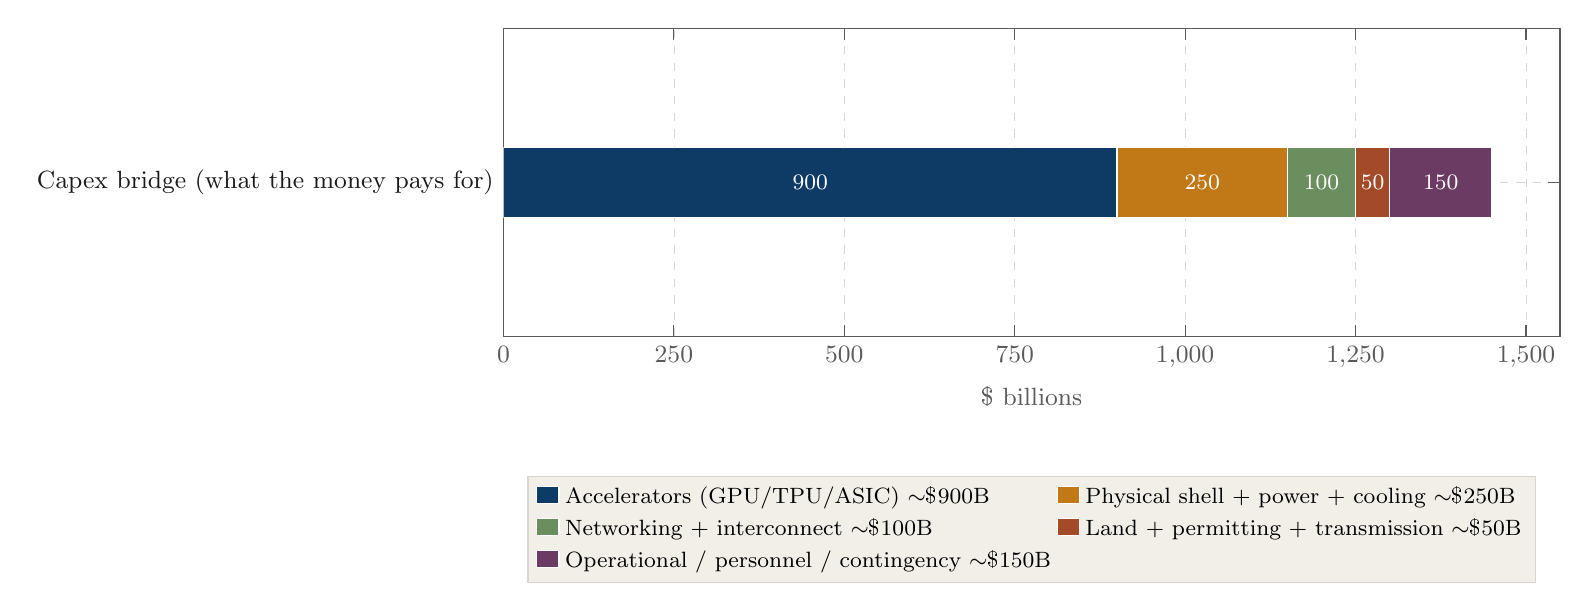
\begin{tikzpicture}
\begin{axis}[
  width=15cm, height=5.5cm,
  xbar stacked,
  bar width=0.9cm,
  enlarge y limits=0.8,
  symbolic y coords={capex},
  ytick=data,
  yticklabels={Capex bridge (what the money pays for)},
  xlabel={\$ billions},
  xlabel style={font=\small,color=softGrey},
  yticklabel style={font=\small,color=inkBlack},
  xticklabel style={font=\small,color=softGrey},
  xmin=0, xmax=1550,
  xtick={0,250,500,750,1000,1250,1500},
  axis line style={softGrey,thin},
  tick style={softGrey,thin},
  grid=major, grid style={paleGrey,dashed,very thin},
  legend style={at={(0.5,-0.45)},anchor=north,font=\footnotesize,draw=paleGrey,fill=lightCream,legend columns=2},
  legend cell align={left},
  nodes near coords,
  nodes near coords style={font=\footnotesize,color=white,align=center},
  every node near coord/.append style={/pgf/number format/.cd,fixed,precision=0},
]
\addplot[fill=chartA,draw=white] coordinates {(900,capex)};
\addlegendentry{Accelerators (GPU/TPU/ASIC) $\sim$\$900B}
\addplot[fill=chartB,draw=white] coordinates {(250,capex)};
\addlegendentry{Physical shell + power + cooling $\sim$\$250B}
\addplot[fill=chartC,draw=white] coordinates {(100,capex)};
\addlegendentry{Networking + interconnect $\sim$\$100B}
\addplot[fill=chartD,draw=white] coordinates {(50,capex)};
\addlegendentry{Land + permitting + transmission $\sim$\$50B}
\addplot[fill=chartE,draw=white] coordinates {(150,capex)};
\addlegendentry{Operational / personnel / contingency $\sim$\$150B}
\end{axis}
\end{tikzpicture}
\caption{Figure 8A. Capex bridge for the Western 2026--2030 \$1.2--1.5T envelope. Accelerator silicon is the dominant share (approximately 60\%) because per-chip ASPs in the B300/Rubin/Trainium-3 era exceed \$30--50k per unit and cluster densities have risen to 1{,}000+~H100e/MW. Physical shell, power, and cooling together are approximately 17\%; networking (intra- and inter-DC) is 7\%; land + permitting + transmission is 3\%; operational, personnel, and execution contingency absorbs the remaining 10\%. Ranges reflect vendor-specific ASP uncertainty and the silicon-uplift sensitivity in \S\ref{subsec:h100e-sensitivity}.\protect\footnotemark}
\end{figure}
\footnotetext{Author's aggregation. Accelerators: per-row \texttt{capex\_bridge.accelerator\_usd\_b} in \texttt{compute\_commitments\_overlay.yaml}, extrapolated to the 51.9~GW facility horizon at blended \$17--20~M per facility-MW. Physical shell + power + cooling: \$44~B/GW Epoch infrastructure benchmark applied to the non-Epoch overlay with \$30~B/GW Epoch benchmark for the Epoch floor. Networking, land, and contingency: \$1.5--3~M/MW per rev-2 appendix audit.}

\textbf{The \$550B RPO is revenue underwriting, not a funding channel.} Between the capex bridge (Figure~8A, what the money physically buys) and the financing bridge (Figure~8B, where the money comes from) lies the \$550B in contracted remaining performance obligations disclosed in the hyperscaler and neocloud 10-K filings. Oracle's \$300B from OpenAI, Anthropic's \$100B+ from Amazon, Anthropic's \$52--60B from Google, Nebius's \$27B from Meta, Nebius's \$19.4B from Microsoft, and CoreWeave's approximately \$50B from Microsoft and OpenAI together constitute \emph{revenue} commitments from labs to infrastructure providers. That revenue backing is what enables the infrastructure provider's SPV or corporate debt to be wrapped to investment grade --- it is the credit-enhancement spine of the debt channel in Figure~8B, not a stand-alone funding bucket.

\begin{figure}[h]
\centering
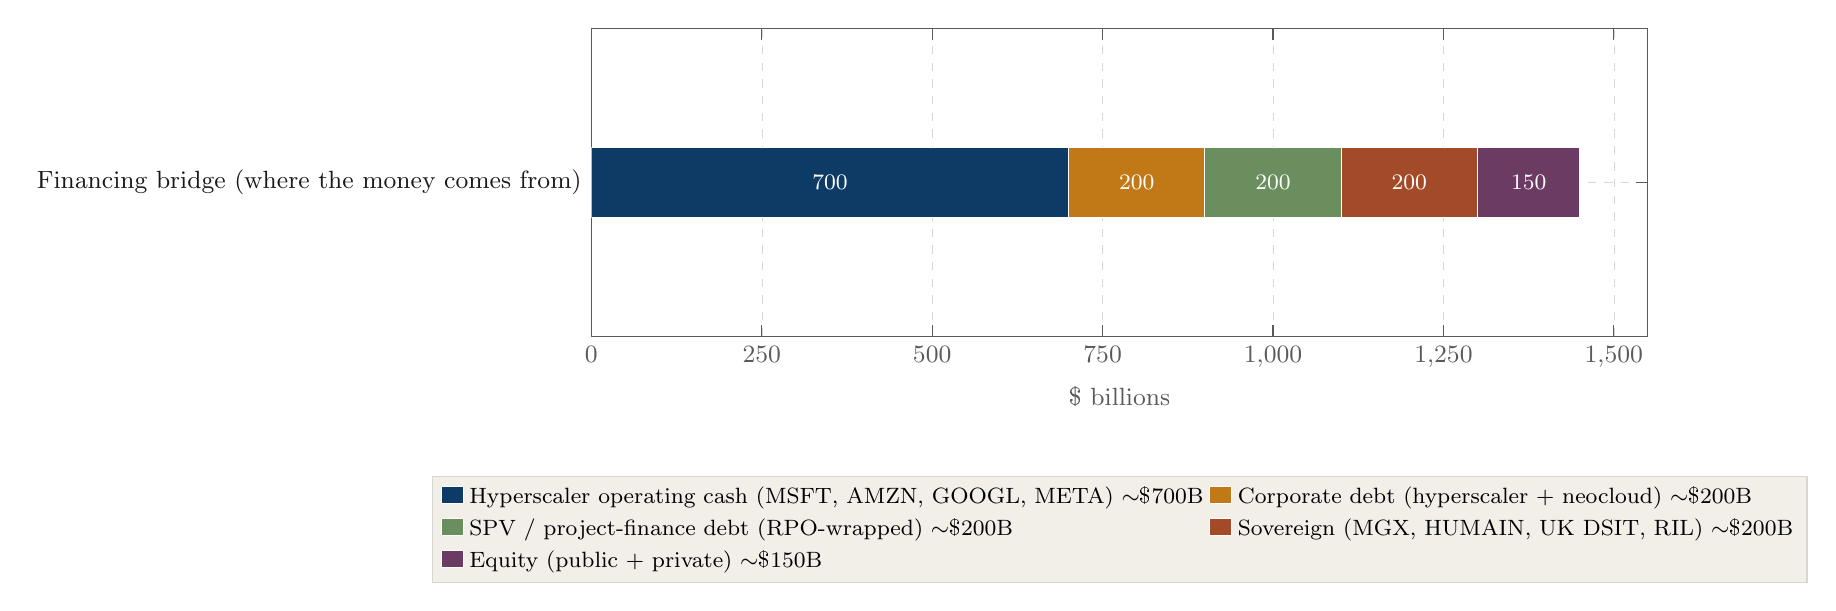
\begin{tikzpicture}
\begin{axis}[
  width=15cm, height=5.5cm,
  xbar stacked,
  bar width=0.9cm,
  enlarge y limits=0.8,
  symbolic y coords={financing},
  ytick=data,
  yticklabels={Financing bridge (where the money comes from)},
  xlabel={\$ billions},
  xlabel style={font=\small,color=softGrey},
  yticklabel style={font=\small,color=inkBlack},
  xticklabel style={font=\small,color=softGrey},
  xmin=0, xmax=1550,
  xtick={0,250,500,750,1000,1250,1500},
  axis line style={softGrey,thin},
  tick style={softGrey,thin},
  grid=major, grid style={paleGrey,dashed,very thin},
  legend style={at={(0.5,-0.45)},anchor=north,font=\footnotesize,draw=paleGrey,fill=lightCream,legend columns=2},
  legend cell align={left},
  nodes near coords,
  nodes near coords style={font=\footnotesize,color=white,align=center},
  every node near coord/.append style={/pgf/number format/.cd,fixed,precision=0},
]
\addplot[fill=chartA,draw=white] coordinates {(700,financing)};
\addlegendentry{Hyperscaler operating cash (MSFT, AMZN, GOOGL, META) $\sim$\$700B}
\addplot[fill=chartB,draw=white] coordinates {(200,financing)};
\addlegendentry{Corporate debt (hyperscaler + neocloud) $\sim$\$200B}
\addplot[fill=chartC,draw=white] coordinates {(200,financing)};
\addlegendentry{SPV / project-finance debt (RPO-wrapped) $\sim$\$200B}
\addplot[fill=chartD,draw=white] coordinates {(200,financing)};
\addlegendentry{Sovereign (MGX, HUMAIN, UK DSIT, RIL) $\sim$\$200B}
\addplot[fill=chartE,draw=white] coordinates {(150,financing)};
\addlegendentry{Equity (public + private) $\sim$\$150B}
\end{axis}
\end{tikzpicture}
\caption{Figure 8B. Financing bridge for the same \$1.2--1.5T capital envelope, decomposed by source of funds. Hyperscaler operating cash flow is the dominant channel (approximately 48\%) because Microsoft, Amazon, Google, and Meta collectively generate roughly \$400B of annual free cash flow before capex. Corporate and SPV debt together add approximately 28\%; the SPV channel is structured against 15-year take-or-pay RPO, wrapped to investment-grade at the SPV level, and issued into private-credit markets. Sovereign capital from MGX, HUMAIN, UK DSIT, and Reliance contributes approximately 14\%. Equity (public markets + private rounds) absorbs the remaining 10\%. The \$550B RPO does \emph{not} appear as a stand-alone channel here --- it is the revenue underwriting that enables the SPV/project-finance debt channel.\protect\footnotemark}
\end{figure}
\footnotetext{Author's aggregation. Hyperscaler channel: Big-Four CY2025 actual plus CY2026 guidance times AI share, extended 2027--2030 at roughly flat dollar levels. Corporate debt: hyperscaler balance-sheet additions plus CoreWeave, Nebius, Applied Digital, Crusoe corporate issuance. SPV / project-finance: Applied Digital--CoreWeave SPV, CoreWeave Blackstone facility, Nebius ABS, Crusoe ABS --- all wrapped to investment-grade via lab-revenue RPO. Sovereign: MGX \$100--200B per OpenAI Stargate announcement + HUMAIN \$10B AMD JV + UK DSIT £5B + RIL estimated \$30--50B Jamnagar phase-one. Equity: OpenAI secondary rounds, Anthropic Series F/G, CoreWeave public-float, Nebius AMS float.}

% ============================================================================
\section{The counterparty graph}
% ============================================================================

Behind the aggregate capex figure sits a strikingly \textbf{concentrated counterparty graph}. Four clusters organise the 2030 Western horizon, with limited bridging between them.

\subsection{Cluster 1: Microsoft--OpenAI--CoreWeave--Oracle}

The largest cluster by 2030 committed GW. Microsoft serves as OpenAI's primary API cloud through January 2030 for first-party workloads. Microsoft hosts roughly \textbf{3--4 GW of OpenAI's aggregate committed compute} inside the Fairwater and Azure programmes. Oracle is the operator of the eight-site Stargate programme, with the \$300 billion take-or-pay commitment from OpenAI anchoring roughly \textbf{10--11 GW of dedicated Stargate build}. CoreWeave provides additional OpenAI capacity under the March 2025 contract (approximately 250 MW of committed capacity, scheduled to grow), and serves Microsoft with a dedicated fleet.\footnote{CoreWeave, Inc.\ and OpenAI, joint press release, March 10, 2025, disclosing a \$11.9 billion five-year agreement. \url{https://www.coreweave.com/news}; CoreWeave Inc.\ and Microsoft Corporation, agreement initially disclosed September 2023 and expanded through 2025.}

\begin{figure}[h]
\centering
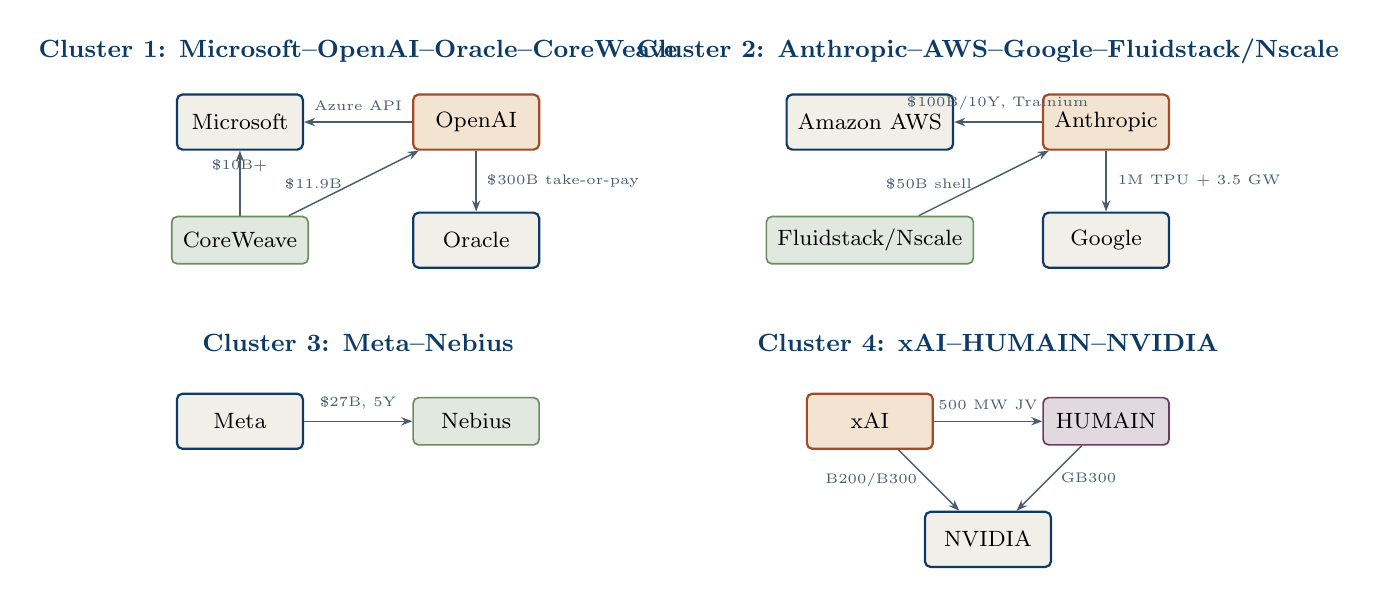
\begin{tikzpicture}[
  every node/.style={font=\footnotesize,inner sep=4pt,rounded corners=2pt},
  hub/.style={fill=lightCream,draw=deepNavy,line width=0.8pt,minimum width=1.6cm,minimum height=0.7cm,align=center},
  lab/.style={fill=accentOchre!20,draw=accentTerracotta,line width=0.8pt,minimum width=1.6cm,minimum height=0.7cm,align=center},
  neocloud/.style={fill=accentSage!20,draw=accentSage,line width=0.6pt,minimum width=1.6cm,minimum height=0.6cm,align=center},
  sov/.style={fill=accentPlum!20,draw=accentPlum,line width=0.6pt,minimum width=1.6cm,minimum height=0.6cm,align=center},
  e/.style={-{Stealth[length=4pt]},line width=0.5pt,color=mutedSlate},
]
% Cluster 1 (MSFT-OpenAI-CW-Oracle) -- top left
\node[hub]     (MSFT) at (0,3)   {Microsoft};
\node[lab]     (OAI)  at (3,3)   {OpenAI};
\node[hub]     (ORCL) at (3,1.5) {Oracle};
\node[neocloud](CW)   at (0,1.5) {CoreWeave};

\draw[e] (OAI) -- node[above,font=\tiny]{Azure API} (MSFT);
\draw[e] (OAI) -- node[right,font=\tiny]{\$300B take-or-pay} (ORCL);
\draw[e] (CW)  -- node[left,font=\tiny]{\$11.9B} (OAI);
\draw[e] (CW)  -- node[above,font=\tiny]{\$10B+} (MSFT);

\node[font=\small\bfseries\color{deepNavy},align=center] at (1.5,3.9)
  {Cluster 1: Microsoft--OpenAI--Oracle--CoreWeave};

% Cluster 2 (Anthropic-AWS-Google-Fluidstack) -- top right
\node[hub]     (AWS)   at (8,3)    {Amazon AWS};
\node[lab]     (ANT)   at (11,3)   {Anthropic};
\node[hub]     (GOOG)  at (11,1.5) {Google};
\node[neocloud](FLX)   at (8,1.5)  {Fluidstack/Nscale};

\draw[e] (ANT) -- node[above,font=\tiny]{\$100B/10Y, Trainium} (AWS);
\draw[e] (ANT) -- node[right,font=\tiny]{1M TPU + 3.5 GW} (GOOG);
\draw[e] (FLX) -- node[left,font=\tiny]{\$50B shell} (ANT);

\node[font=\small\bfseries\color{deepNavy},align=center] at (9.5,3.9)
  {Cluster 2: Anthropic--AWS--Google--Fluidstack/Nscale};

% Cluster 3 (Meta-Nebius) -- bottom left
\node[hub]     (META)  at (0,-0.8)   {Meta};
\node[neocloud](NEB)   at (3,-0.8)   {Nebius};

\draw[e] (META) -- node[above,font=\tiny]{\$27B, 5Y} (NEB);

\node[font=\small\bfseries\color{deepNavy},align=center] at (1.5,0.2)
  {Cluster 3: Meta--Nebius};

% Cluster 4 (xAI-HUMAIN-NVIDIA) -- bottom right
\node[lab]   (XAI)    at (8,-0.8)   {xAI};
\node[sov]   (HUM)    at (11,-0.8)  {HUMAIN};
\node[hub]   (NVDA)   at (9.5,-2.3) {NVIDIA};

\draw[e] (XAI) -- node[above,font=\tiny]{500 MW JV} (HUM);
\draw[e] (XAI) -- node[left,font=\tiny]{B200/B300} (NVDA);
\draw[e] (HUM) -- node[right,font=\tiny]{GB300} (NVDA);

\node[font=\small\bfseries\color{deepNavy},align=center] at (9.5,0.2)
  {Cluster 4: xAI--HUMAIN--NVIDIA};
\end{tikzpicture}
\caption{Schematic of the four principal counterparty clusters in the 2026--2030 Western compute horizon. Edges are labelled with the dominant dollar-value or physical-capacity commitment between each pair. The bridging links between clusters (e.g., Anthropic on Microsoft Azure; xAI on Oracle/Microsoft) are omitted for clarity but represent roughly 15\% of each cluster's aggregate exposure.\protect\footnotemark}
\end{figure}
\footnotetext{Counterparty values from individual cited announcements throughout this paper. The graph is not complete (omitting, e.g., Meta's relationship with its own internal silicon roadmap, and Microsoft's additional third-party-lab partnerships) but captures the material dollar commitments governing the 2030 horizon.}

\subsection{Concentration risk}

CoreWeave disclosed in its FY2025 10-K that \textbf{two customers collectively account for 77\% of revenue}, with Microsoft alone at 62\%.\footnote{CoreWeave FY2025 10-K, ``Revenue Concentration'' risk factor: ``For the year ended December 31, 2025, Microsoft represented 62\% of our revenue, and our second-largest customer represented approximately 15\%.''} Nebius's disclosed aggregate RPO of approximately \$46 billion sits on two counterparties (Meta \$27~B, Microsoft \$19~B, with smaller residuals). The sovereign programmes in HUMAIN, MGX, and RIL each have a single anchor tenant. The neocloud segment as a whole is therefore \textbf{materially concentrated on five investment-grade counterparties} (Microsoft, Meta, OpenAI-via-Microsoft, Amazon-through-Anthropic, Google), and any individual counterparty pause or re-scoping would transmit directly to the merchant-neocloud capex plan.

% ============================================================================
\section{Execution risk: what breaks the build-out}
% ============================================================================

\textbf{Approximately 85\% of the 51.9~GW facility raw horizon is not yet operational; probability-weighted expected realization by 2030 is approximately 36.8~GW facility, of which roughly 78\% is not yet operational today.} The build-out is therefore a forward execution bet, not an in-place compute base. The principal risks are concentrated in four categories: grid interconnection, chip delivery, counterparty concentration, and the realisation of outer-year stretch targets (particularly Meta Hyperion, Reliance Jamnagar, and the Anthropic--Amazon full 5~GW). Each is priced into the stress-scenario matrix in \S\ref{subsec:stress-matrix}.

\subsection{Confidence decomposition of the 2030 horizon}

Of the 51.9~GW facility Western horizon, the six-tier evidence split is: \textbf{T1 Operational} 15\% (7.56~GW, 100\% realization), \textbf{T2 Under construction / physically evidenced} 24\% (12.43~GW, 88\% default), \textbf{T3 Firm commercial} 15\% (7.95~GW, 78\% default), \textbf{T4 Announced site-level plan} 33\% (16.91~GW, 58\% default), \textbf{T5 LOI / stretch target} 13\% (6.75~GW, 32\% default), and \textbf{T6 Analyst inference} 1\% (0.33~GW, 25\% default). Probability-weighted sum across the six tiers yields approximately \textbf{36.8~GW facility} as the deterministic expected 2030 realization --- materially below the 51.9~GW announced horizon and materially above the 27.9~GW conservative case (T1+T2+T3 only). The Monte Carlo median (\S\ref{subsec:monte-carlo}) at approximately 31.8~GW facility is our probability-honest base case.

\begin{figure}[h]
\centering
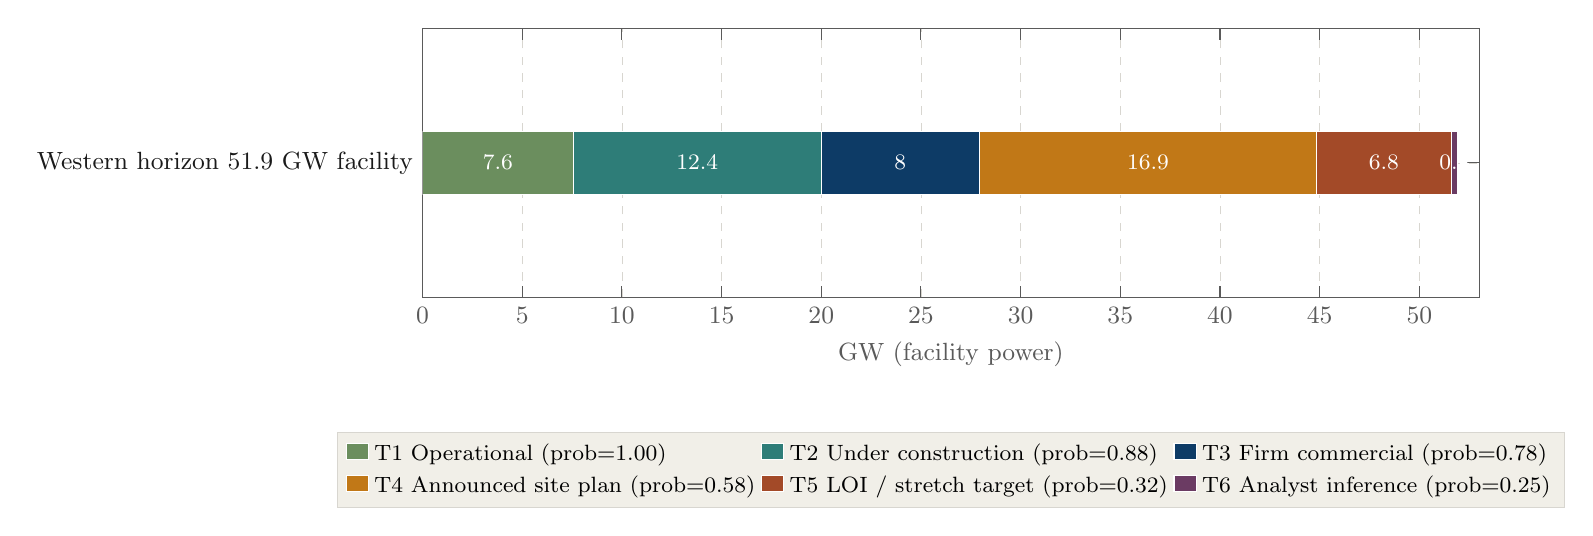
\begin{tikzpicture}
\begin{axis}[
  width=15cm, height=5cm,
  xbar stacked,
  bar width=0.8cm,
  enlarge y limits=0.8,
  symbolic y coords={horizon},
  ytick=data,
  yticklabels={Western horizon 51.9 GW facility},
  xlabel={GW (facility power)},
  xlabel style={font=\small,color=softGrey},
  yticklabel style={font=\small,color=inkBlack},
  xticklabel style={font=\small,color=softGrey},
  xmin=0, xmax=53,
  axis line style={softGrey,thin},
  tick style={softGrey,thin},
  grid=major, grid style={paleGrey,dashed,very thin},
  legend style={at={(0.5,-0.5)},anchor=north,font=\footnotesize,draw=paleGrey,fill=lightCream,legend columns=3},
  legend cell align={left},
  nodes near coords,
  nodes near coords style={font=\footnotesize,color=white,align=center},
  every node near coord/.append style={/pgf/number format/.cd,fixed,precision=1},
]
\addplot[fill=accentSage,draw=white] coordinates {(7.56,horizon)};
\addlegendentry{T1 Operational (prob=1.00)}
\addplot[fill=chartG,draw=white] coordinates {(12.43,horizon)};
\addlegendentry{T2 Under construction (prob=0.88)}
\addplot[fill=chartA,draw=white] coordinates {(7.95,horizon)};
\addlegendentry{T3 Firm commercial (prob=0.78)}
\addplot[fill=accentOchre,draw=white] coordinates {(16.91,horizon)};
\addlegendentry{T4 Announced site plan (prob=0.58)}
\addplot[fill=accentTerracotta,draw=white] coordinates {(6.75,horizon)};
\addlegendentry{T5 LOI / stretch target (prob=0.32)}
\addplot[fill=chartE,draw=white] coordinates {(0.33,horizon)};
\addlegendentry{T6 Analyst inference (prob=0.25)}
\end{axis}
\end{tikzpicture}
\caption{Distribution of the 51.9~GW facility Western horizon across six evidence tiers. Per-tier realization probability is the tier-default midpoint with per-row override possible; see \texttt{CONFIDENCE\_DECOMPOSITION.md} for tier definitions and per-row \texttt{realization\_probability} in the overlay YAML. Probability-weighted sum across the six tiers = approximately \textbf{36.8~GW facility} (Figure 10B shows the same segments re-scaled by tier-default probability).\protect\footnotemark}
\end{figure}
\footnotetext{Tier thresholds: \textbf{T1 Operational} = MW online Q2 2026 from Epoch. \textbf{T2 Under construction / physically evidenced} = Epoch sites with active construction visible via satellite or permit and end-of-timeline 2026--2027, plus the 0.70~GW Fairwater-international overlay (Narvik/Loughton/Dublin). \textbf{T3 Firm commercial} = 15-year take-or-pay contracts with investment-grade counterparties (CoreWeave--Microsoft, CoreWeave--OpenAI, Nebius--Meta, Applied Digital--CoreWeave SPV). \textbf{T4 Announced site-level plan} = Epoch sites scheduled 2028 plus overlay commitments with named site, operator, MW, primary-source-backed (Anthropic-AWS 3.17~GW incremental, Stargate 10~GW, xAI-HUMAIN 0.5~GW). \textbf{T5 LOI / stretch target} = Epoch 2029--2030 speculative plus the Meta Hyperion 2.74~GW stretch delta. \textbf{T6 Analyst inference} = residual xAI Colossus~2 0.06~GW plus the 0.20~GW neocloud-ex-Epoch analyst inference.}

\begin{figure}[h]
\centering
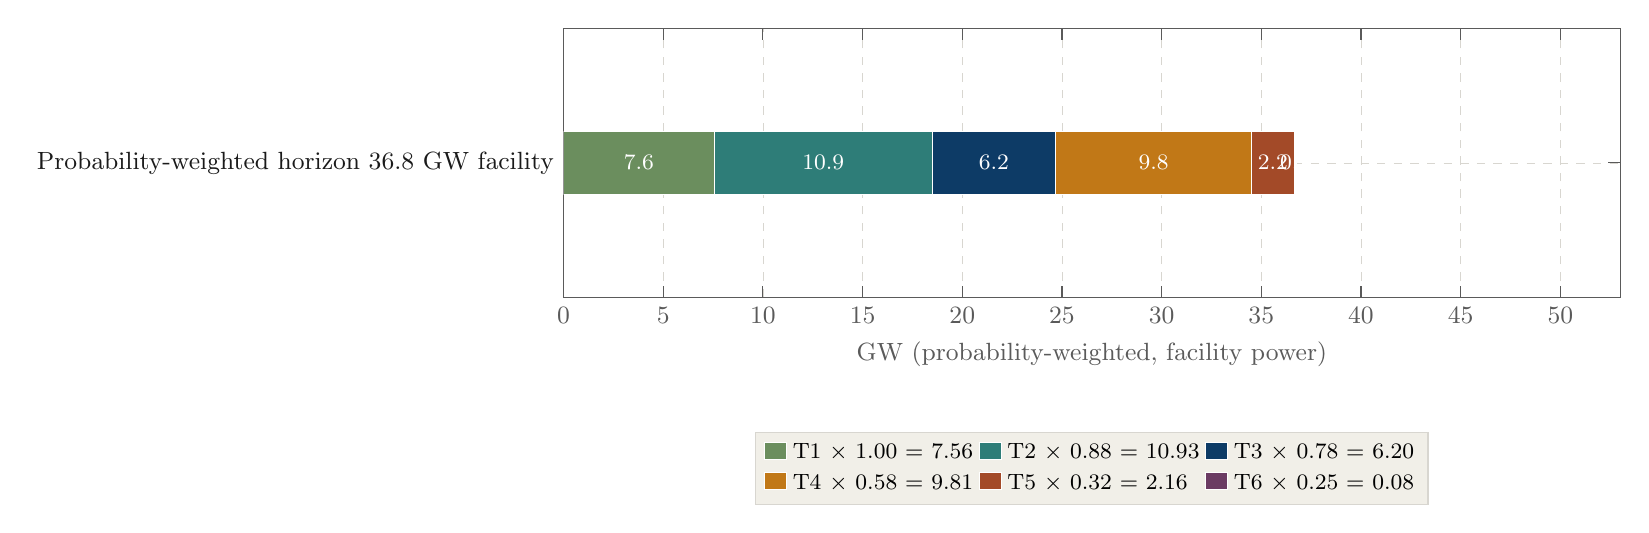
\begin{tikzpicture}
\begin{axis}[
  width=15cm, height=5cm,
  xbar stacked,
  bar width=0.8cm,
  enlarge y limits=0.8,
  symbolic y coords={horizon},
  ytick=data,
  yticklabels={Probability-weighted horizon 36.8 GW facility},
  xlabel={GW (probability-weighted, facility power)},
  xlabel style={font=\small,color=softGrey},
  yticklabel style={font=\small,color=inkBlack},
  xticklabel style={font=\small,color=softGrey},
  xmin=0, xmax=53,
  axis line style={softGrey,thin},
  tick style={softGrey,thin},
  grid=major, grid style={paleGrey,dashed,very thin},
  legend style={at={(0.5,-0.5)},anchor=north,font=\footnotesize,draw=paleGrey,fill=lightCream,legend columns=3},
  legend cell align={left},
  nodes near coords,
  nodes near coords style={font=\footnotesize,color=white,align=center},
  every node near coord/.append style={/pgf/number format/.cd,fixed,precision=1},
]
\addplot[fill=accentSage,draw=white] coordinates {(7.56,horizon)};
\addlegendentry{T1 $\times$ 1.00 = 7.56}
\addplot[fill=chartG,draw=white] coordinates {(10.93,horizon)};
\addlegendentry{T2 $\times$ 0.88 = 10.93}
\addplot[fill=chartA,draw=white] coordinates {(6.20,horizon)};
\addlegendentry{T3 $\times$ 0.78 = 6.20}
\addplot[fill=accentOchre,draw=white] coordinates {(9.81,horizon)};
\addlegendentry{T4 $\times$ 0.58 = 9.81}
\addplot[fill=accentTerracotta,draw=white] coordinates {(2.16,horizon)};
\addlegendentry{T5 $\times$ 0.32 = 2.16}
\addplot[fill=chartE,draw=white] coordinates {(0.08,horizon)};
\addlegendentry{T6 $\times$ 0.25 = 0.08}
\end{axis}
\end{tikzpicture}
\caption{Figure 10B. Same six tiers as Figure 10, with each segment re-scaled by its tier-default realization probability. The expected 2030 Western realization is approximately \textbf{36.8~GW facility} --- the right-hand edge of the stacked bar. This is our deterministic base case; the Monte Carlo median is approximately 31.8~GW facility (\S\ref{subsec:monte-carlo}). The T1+T2+T3 conservative subset (7.56 + 10.93 + 6.20 = 24.7~GW expected, or 27.9~GW announced facility) sits as the conservative reading; the 55.3~GW facility arithmetic ceiling as the full-realization case. Rev-3: basis is now facility power (rev-2 used IT-load; see \S\ref{subsec:power-units}).}
\end{figure}

\subsection{Scenario ranges: non-stretch 45.2 GW to full-realization 55.3 GW (facility)}

Stripping the stretch-target-only tier (T5) and compressing speculative completions yields a \textbf{raw non-stretch reading} of approximately \textbf{45.2~GW facility} (announced minus T5). Realising every stretch on disclosed timeline yields a \textbf{full-realization ceiling} of approximately \textbf{55.3~GW facility}. The deterministic tier-weighted base of \textbf{36.8~GW facility} sits between the two because tier-default probabilities discount each tier. The Monte Carlo median (\S\ref{subsec:monte-carlo}) falls lower still at approximately \textbf{31.8~GW facility}, reflecting the joint effect of per-tier realization variance and correlated stress scenarios.

\subsection{The grid is the binding constraint in the out-years}

Chip-vendor delivery slippage has historically compressed site-level buildout timelines by three to nine months per generation; NVIDIA Blackwell shipped approximately four months behind its original schedule, and Rubin appears to be tracking to its original late-2026 availability.\footnote{NVIDIA Corporation, Q4 FY2026 earnings, February 26, 2026, Jensen Huang commentary on Rubin shipping commencement: ``Rubin will begin revenue shipments in Q2 calendar 2026, in line with our prior guidance.''} Grid interconnection slippage, by contrast, is structural and approximately \textbf{18 to 30 months on the scheduled interconnect date}, with no comparable compensatory mechanism on the utility side. The combined effect is that \textbf{2028--2029 buildouts carry substantially higher grid-slippage risk than chip-delivery risk}, particularly for the 8--9 GW of the horizon sited in grid-constrained footprints (Northern Virginia residual, the ERCOT West Texas queue, the MISO large-load queue in Wisconsin and Ohio).

\subsection{Stress scenarios: five transmission mechanisms that move the horizon}
\label{subsec:stress-matrix}

The 51.9~GW facility announced horizon, 36.8~GW facility probability-weighted horizon, and 27.9~GW facility conservative horizon are single-path point estimates. The more decision-relevant question is: which individual mechanisms, if they realize, materially move any of those numbers? We identify five named stress scenarios, each with an estimated GW impact, a capex-envelope impact, named counterparties most exposed, and an assigned probability.

\begin{table}[h]
\centering
\small
\renewcommand{\arraystretch}{1.25}
\begin{tabular}{@{}p{3.3cm}rrp{4.4cm}r@{}}
\toprule
\textbf{Scenario} & \textbf{$\Delta$GW 2030} & \textbf{$\Delta$\$B capex} & \textbf{Counterparties affected} & \textbf{Prob.} \\
\midrule
A. Stargate 12-month slip & $-3.5$ & $-120$ & Oracle, MSFT, CoreWeave, SoftBank & 30\% \\
B. Neocloud spread widen 300bps & $-2.0$ & $-60$ & CoreWeave, Nebius, Applied Digital, Crusoe & 25\% \\
C. Grid 24-mo slip ERCOT/MISO/PJM & $-8.0$ & $-180$ & broad; xAI, Meta, Stargate most & 40\% \\
D. NVIDIA/TPU/Trainium 2Q slip & $-1.5$ & $-40$ & all Class A & 50\% \\
E. Inference outpaces training & $0.0$ & $-20$ & chip-family mix shift & 55\% \\
\bottomrule
\end{tabular}
\caption{Five named stress scenarios. GW deltas are point estimates of impact on the 2030 Western horizon under each scenario in isolation. The probability column is the probability that the \emph{scenario realizes at all}, not a conditional probability on any particular outcome. Correlated-shock cases (e.g.\ A+B+C simultaneously) are not summed here; see prose below.}
\end{table}

\textbf{Scenario A (Stargate 12-month slip, 30\% prob).} The eight-site Stargate programme represents roughly 10.6~GW of the Western horizon. A 12-month slip across the outer-phase sites (Shackelford, Lordsburg, Milam, Do{\~n}a Ana) from the announced 2028 scheduled online to 2029 reduces 2030 realized GW by approximately 3.5~GW and removes approximately \$120~B of 2028--2030 capex recognition. Transmission: any combination of ERCOT/PJM queue delay, Oracle financing disruption, or OpenAI-Microsoft restructuring friction.

\textbf{Scenario B (Neocloud spread widen 300bps, 25\% prob).} A shock to neocloud senior-secured debt spreads from today's 250--400~bps to 550--700~bps removes roughly 2~GW of marginal 2028--2030 buildout, concentrated in Applied Digital / Crusoe / Voltage Park tier operators whose financing is most sensitive. Transmission: concentrated-counterparty default (e.g.\ lab-revenue disappointment cascading through CoreWeave), broader credit-cycle widening, or a single large-project write-down.

\textbf{Scenario C (Grid 24-month slip across ERCOT/MISO/PJM, 40\% prob).} The largest single scenario risk. A 24-month slip in new transmission and substation delivery across the three ISOs holding roughly 30~GW of the horizon would push 2028--2030 scheduled GW into 2030--2032, removing approximately 8~GW from the 2030 realized reading and approximately \$180~B of capex. This is Scenario C priced at the highest probability (40\%) because the structural imbalance between queue length and deliverable transmission is already visible in public queue reports.

\textbf{Scenario D (Chip vendor 2-quarter slip, 50\% prob).} NVIDIA Rubin, AWS Trainium~4, or Google TPU~v8 slips from the currently-guided availability by two quarters. GW impact is small (1.5~GW, concentrated in outer-phase 2029--2030 cluster commissioning) but H100e impact is larger (12M H100e, or roughly 15\% of the base silicon-uplift reading). This is priced at 50\% probability because chip-vendor slip is historically the most frequent of the five.

\textbf{Scenario E (Inference outpaces training, 55\% prob).} Not a GW scenario but a chip-mix scenario. If late-2020s frontier demand is dominated by inference workloads (agentic workflows, real-time serving) rather than training, the silicon mix shifts toward inference-optimized families (Trainium-inference, MTIA~v2, Groq, Google TPU~v8i) and away from training-optimized Blackwell/Rubin. The physical GW stays the same but chip dollars rotate roughly 15--25\% away from NVIDIA. Probability is 55\% because at least partial inference-share expansion is consensus; the uncertainty is degree.

\textbf{The correlated case.} A+B+C together --- Stargate slip, spread widening, grid-queue slip --- is not modelled as a single scenario because the correlation structure is unstable. Conservatively, the three scenarios together would remove 10--12~GW from the 2030 realized horizon and \$300--350~B from the capex envelope; this is the realistic downside reading that sits below our conservative 27.9~GW facility case and is the scenario an LP would properly stress-test against.

\subsection{Monte Carlo: distribution of the 2030 realized horizon}
\label{subsec:monte-carlo}

The tier-deterministic 36.8~GW facility probability-weighted horizon is a single point. The more decision-relevant question is the \emph{shape} of the 2030 realization distribution, which requires combining tier-level sampling with the stress-scenario realizations. The companion \texttt{monte\_carlo\_horizon.py} script runs 10{,}000 draws per invocation: per tier, realization rate is sampled from a Beta fitted so the tier default is the mean and the documented variance bracket is p05--p95 (T1 fixed at 1.00; T2 Beta[0.80, 0.95]; T3 Beta[0.65, 0.90]; T4 Beta[0.40, 0.75]; T5 Beta[0.15, 0.50]; T6 Beta[0.10, 0.40]); each of the five stress scenarios independently fires with its assigned probability and, if fired, subtracts its GW delta.

\begin{table}[h]
\centering
\small
\begin{tabular}{@{}lr@{}}
\toprule
\textbf{Percentile of 2030 realized GW (facility)} & \textbf{GW} \\
\midrule
p05 (5th percentile) & 23.1 \\
p10 & 24.6 \\
p25 & 27.5 \\
p50 (median) & 31.8 \\
p75 & 35.3 \\
p90 & 37.4 \\
p95 & 38.4 \\
\midrule
Mean & 31.3 \\
Std.\ dev. & 4.9 \\
\bottomrule
\end{tabular}
\caption{Monte Carlo distribution of the 2030 Western realized horizon (facility basis), 10{,}000 draws. Seed 20260424, rev-3 tier rollup (T1=7.56, T2=12.43, T3=7.95, T4=16.91, T5=6.75, T6=0.33 facility). \textbf{The sim median (31.8~GW facility) sits approximately 5~GW below the tier-deterministic 36.8~GW facility} because the stress-scenario stack has negative expected value: A+B+C+D together carry an unconditional expected GW loss of approximately $-5.9$~GW ($-3.5 \cdot 0.30 - 2.0 \cdot 0.25 - 8.0 \cdot 0.40 - 1.5 \cdot 0.50$). Readers treating the deterministic 36.8~GW as central estimate should shift that estimate down by roughly 5~GW to recover a probability-honest central value. IT-load bridge: MC median 31.1~GW IT (see \S\ref{subsec:power-units}).}
\end{table}

\textbf{Tail probabilities from the sim (facility basis):}
\begin{itemize}\itemsep0pt
\item $P(\text{realized 2030 GW} < 27.9$ conservative case$) \approx 28\%$
\item $P(\text{realized 2030 GW} < 36.8$ tier-deterministic$) \approx 86\%$
\item $P(\text{realized 2030 GW} < 45.2$ raw non-stretch$) = 100\%$
\item $P(\text{realized 2030 GW} < 51.9$ announced horizon$) = 100\%$
\end{itemize}

The reader's practical takeaway: \textbf{our base case is the Monte Carlo median of approximately 31.8~GW facility with a p10--p90 interdecile range of $[24.6, 37.4]$~GW facility}, not the naive tier-weighted 36.8~GW point. The announced 51.9~GW and the raw non-stretch 45.2~GW are both above the full simulation's p95 --- no scenario-plausible distribution realizes either figure. The conservative 27.9~GW T1+T2+T3 case is an approximately p28 event: plausible but not central. An LP stress-testing this forecast should focus on p10 (approximately 24.6~GW facility) as the stressed-but-plausible reading, not on the announced horizon or the tier-deterministic point.

% ============================================================================
\section{Sovereign AI}
% ============================================================================

The sovereign-AI pipeline is reported separately from the Western-aligned horizon because state-backed programmes operate under different financing, revenue-model, and timeline dynamics. Four programmes dominate the 2030 sovereign pipeline, each labeled with its evidence tier and realization probability on the same 6-tier framework applied to the Western denominator: \textbf{UAE G42-Khazna / Stargate UAE} --- Phase 1 200~MW \textbf{(T1 operational, prob=1.00)}; expansion to 1~GW by 2030 \textbf{(T4 announced, prob=0.70)}. \textbf{Saudi HUMAIN--AMD} --- 500~MW over 5 years \textbf{(T4, prob=0.55)}. \textbf{Saudi HUMAIN--xAI} --- 500~MW JV, Phase 1 cluster \textbf{(T4, prob=0.55)}. \textbf{UK Culham AI Growth Zone} --- 500~MW by 2030, initial 100--250~MW by 2027 \textbf{(T5 stretch, no anchor tenant disclosed yet, prob=0.30)}. \textbf{India Reliance Jamnagar} --- Phase 1 120~MW H2 2026 \textbf{(T1--T2, prob=0.95)}; ``gigawatt-scale'' AGM target \textbf{(T5 stretch, prob=0.20)}. \textbf{Sovereign sum: 2.06~GW facility announced (1.95~GW IT-load bridge), 0.70~GW facility probability-weighted.} This is not additive to the Western 51.9~GW facility denominator.

\begin{figure}[h]
\centering
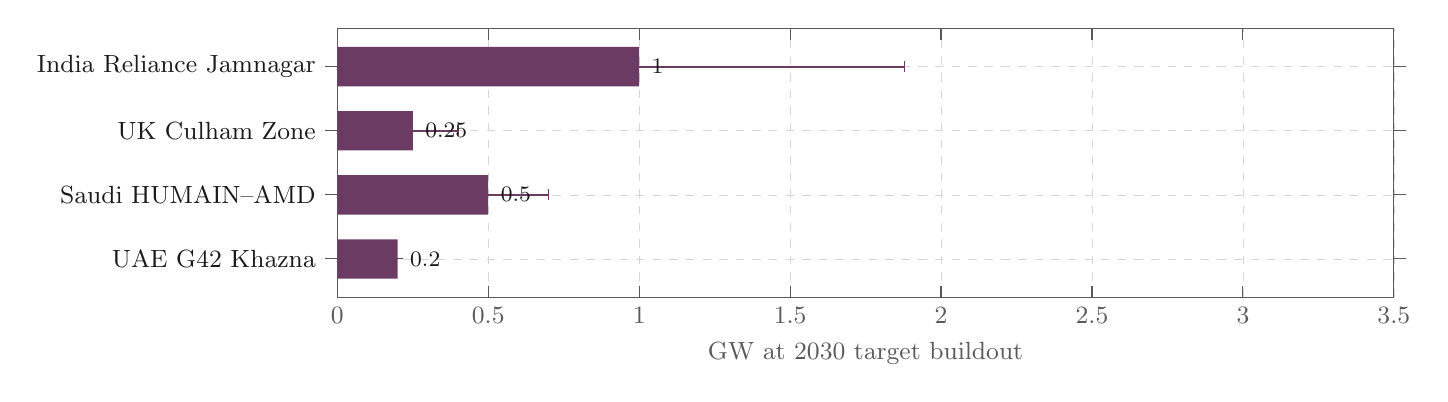
\begin{tikzpicture}
\begin{axis}[
  width=15cm, height=5cm,
  xbar,
  bar width=0.5cm,
  enlarge y limits=0.2,
  symbolic y coords={UAE,Saudi,UK,India},
  ytick=data,
  yticklabels={UAE G42 Khazna,Saudi HUMAIN--AMD,UK Culham Zone,India Reliance Jamnagar},
  xlabel={GW at 2030 target buildout},
  xlabel style={font=\small,color=softGrey},
  yticklabel style={font=\small,color=inkBlack},
  xticklabel style={font=\small,color=softGrey},
  xmin=0, xmax=3.5,
  axis line style={softGrey,thin},
  tick style={softGrey,thin},
  grid=major, grid style={paleGrey,dashed,very thin},
  nodes near coords,
  nodes near coords style={font=\footnotesize,color=inkBlack,anchor=west,xshift=1pt},
  nodes near coords align={horizontal},
]
\addplot[fill=chartE,draw=none,
         error bars/.cd,
         x dir=both,x explicit,
         error bar style={line width=0.8pt,color=accentPlum}]
  coordinates {
    (0.20,UAE) +- (0, 0)
    (0.50,Saudi) +- (0.20, 0.20)
    (0.25,UK) +- (0.15, 0.25)
    (1.00,India) +- (0.88, 2.00)
  };
\end{axis}
\end{tikzpicture}
\caption{Sovereign-AI pipeline, 2030 target GW with low-high ranges. \textbf{Unit:} GW at commissioning (mixed IT / facility basis; per-row flag in overlay YAML). \textbf{Tier labels:} UAE = T1 Phase~1 + T4 expansion (prob=1.00 + 0.70); Saudi HUMAIN--AMD = T4 (prob=0.55); UK Culham = T5 (prob=0.30); India Reliance = T1--T2 Phase~1 + T5 stretch (prob=0.95 + 0.20). \textbf{Aggregate:} 2.06~GW facility announced (1.95~GW IT-load bridge), 0.70~GW facility probability-weighted. \textbf{Not included in Western 51.9~GW facility denominator.} Error bars show the range between verifiable floor (Phase-1 commitments) and stated ceiling (AGM / head-of-state language). Reliance Jamnagar carries the widest range because Ambani's 47th AGM language is ``gigawatt-scale'' without specificity; secondary reporting ceilings up to 3~GW.\protect\footnotemark}
\end{figure}
\footnotetext{UAE G42 Khazna: Microsoft, \emph{Microsoft and G42 break ground on UAE-based AI data center with Khazna}, November 1, 2025, firm Phase~1 at 200 MW. Saudi HUMAIN--AMD: AMD, \emph{AMD and HUMAIN announce strategic collaboration}, May 13, 2025, ``500 MW of AI infrastructure deployment over the next 5 years''; \$10 billion JV. UK Culham: UK Government, \emph{AI Opportunities Action Plan}, January 13, 2025, £5 billion commitment. Reliance Jamnagar: Mukesh Ambani, 47th AGM address, August 29, 2024, ``gigawatt-scale AI-ready data centre''; Phase 1 120 MW online H2 2026 per 2026 investor disclosures.}

\subsection{Why the sovereign segment is reported separately}

Three reasons justify the separation. First, \textbf{revenue models are different}: sovereign AI builds are typically anchored on state-directed demand (e.g., Saudi PIF direct consumption, India Reliance consumer services) rather than merchant-cloud markets, which makes the capex-revenue matching logic structurally different from the Western analysis. Second, \textbf{financing is state-backed}: MGX and PIF operate under sovereign-balance-sheet support that changes the effective cost of capital by 200--400~bps below the Western merchant-neocloud market. Third, \textbf{execution timelines are more variable}: grid-connection disputes in Saudi Arabia and India have historically added 12--24 months to announced commissioning schedules.

% ============================================================================
\section{Known unknowns}
% ============================================================================

A forecast is only useful if its author has been explicit about what the forecast does not know. The 6-tier evidence framework in \S\ref{subsec:power-units} and the stress-scenario matrix in \S\ref{subsec:stress-matrix} price in the uncertainty we can structure; this section names the uncertainty we cannot.

\subsection{PUE and facility-versus-IT power ambiguity}

The single largest definitional uncertainty in this paper is whether a given announcement's ``X gigawatts'' refers to IT load at the accelerator, facility power at the utility meter, or reserved interconnection capacity at the substation. Primary-source language is inconsistent: Anthropic's April 20, 2026 ``up to 5~GW of new capacity'' does not specify basis; OpenAI's September 2025 Stargate expansion ``nearly 7 gigawatts'' is implicitly facility power; Microsoft's Fairwater Wisconsin disclosures use ``electrical capacity'' in one press asset and ``IT power'' in another. The paper's per-row \texttt{mw\_basis} field makes the assumption transparent, but when an operator subsequently revises basis, headline horizon numbers move by up to 20\%.

\subsection{Interconnection queue opacity}

ERCOT's large-load queue contains roughly 150~GW of requests against approximately 5~GW per year of deliverable new transmission. MISO, PJM, and Western Interconnection queues are proportionally congested. The paper treats queue position as binary (in-service / approved-no-COD / queued / undetermined) but cannot observe internal queue reshuffling, curtailment conditions attached to conditional approvals, or the bilateral negotiations that determine final COD schedules. For any individual site, this is the largest source of timing risk; for the aggregate, it is priced into Scenario C of the stress-matrix at 40\% probability of a 24-month slip across multiple ISO footprints.

\subsection{Chip roadmap uncertainty post-2027}

Per-chip H100-equivalent density for NVIDIA Rubin, AWS Trainium~4, Google TPU~v8, AMD MI400, Broadcom XPU, and Meta MTIA~v3 is disclosed at roadmap level through 2027 but relies on extrapolation of observed per-family density curves for 2028--2030. If foundation-model compute demand shifts from 8-bit training toward lower-precision (4-bit, 2-bit) or mixed-precision inference workloads, the effective H100-equivalent normalization breaks down and the silicon layer must be re-priced. Our conservative-base-aggressive scenario range (60M / 78M / 110M H100e) is wide because of this.

\subsection{Actual cluster utilization}

Published specifications describe nameplate chip count and nameplate throughput. Actual training-cluster utilization --- the ratio of delivered FLOP-hours to theoretical peak --- is disclosed by almost no operator. Publicly reported efficiency figures from Meta's Llama~3 training paper (38--42\% of peak) and xAI's Colossus training campaign (reportedly 35--45\%) suggest a material gap between nameplate and delivered compute, but these are single data points. The forecast makes no utilization adjustment; any attempt to do so would introduce a further $\pm$20\% uncertainty band that we prefer to leave unpriced.

\subsection{Training-versus-inference mix}

The silicon stack optimal for training (H100/H200/Blackwell/Rubin, with high-bandwidth memory and full-fabric interconnect) diverges increasingly from the stack optimal for inference (Groq, Meta MTIA-v2, AWS Trainium-inference variants, Google TPU-v8i). If late-2020s frontier-model demand tilts further toward inference --- a plausible outcome if agentic workflows and real-time inference become the dominant customer demand --- then the B300/Rubin share of the horizon's chip dollars falls by 10--25\% relative to our base case. Scenario~E in \S\ref{subsec:stress-matrix} prices this at 55\% probability.

\subsection{Double-counting residual risk}

The paper's double-count discipline consolidates at the site level and separates chip commitments (Class~B) from physical-site commitments (Class~A). Residual risk remains in three places: (i) bilateral subleasing between neoclouds and hyperscalers that moves gigawatts between operator lines without appearing in either filing; (ii) overlap between Oracle-operated Stargate and Microsoft-operated Azure where OpenAI workloads land at one site but are billed to the other; (iii) chip commitments where the shell has not yet been identified (e.g., Broadcom's ``10~GW XPU with a named customer'' where press confirmation of Anthropic identity landed three weeks after the shell-level allocation had been modeled). We estimate the residual double-count risk at approximately 2~GW of the 51.9~GW facility horizon, or roughly 4\%.

\subsection{Contract enforceability on take-or-pay}

The \$550~billion of contracted RPO anchoring the Western 2030 horizon is not commercially tested at distress. No Western frontier-lab or hyperscaler counterparty has defaulted on a multi-gigawatt take-or-pay obligation, and the contract documents themselves are not public. In the event of a prolonged lab-revenue disappointment, the enforceability of 15-year take-or-pay contracts against lab counterparties without external revenue backing is legally untested. This is the single most consequential unknown for neocloud creditors (CoreWeave bondholders, Applied Digital SPV lenders, Crusoe ABS investors).

\subsection{Neocloud financing availability under spread-widening}

Merchant-neocloud debt spreads at April 2026 stand at 250--400~bps over Treasuries for senior secured notes collateralized by hyperscaler-contracted revenue. A spread-widening of 300+~bps --- driven by concentrated-counterparty default, a broader credit cycle, or a project-level execution disappointment --- materially constrains the marginal gigawatt of 2028--2030 neocloud buildout. Scenario~B in the stress-matrix prices this at 25\% probability for a 2~GW/\$60~billion impact.

\subsection{Sovereign-AI disclosure asymmetry}

Sovereign programs disclose less than Western hyperscalers and lab counterparties. UAE G42-Khazna uses press-release granularity; Saudi HUMAIN-AMD operates behind confidential PIF-AMD JV terms; India Reliance Jamnagar disclosure is limited to AGM oratory and the 47th AGM Chairman Statement. The 2.06~GW facility sovereign sidebar in this paper is the disclosed floor, not the commissioned ceiling. A doubling or tripling of sovereign build intent in 2027--2028 is plausible and is the largest upside surprise not priced into the Western horizon.

\subsection{China undercount}

The paper deliberately restricts scope to Western-aligned operators and the four named sovereign programs. Chinese AI compute build-out --- Alibaba, ByteDance, Baidu, Tencent, Huawei Ascend, and the CAC-directed sovereign cluster --- is acknowledged to be material (publicly reported intent is in the 20--40~GW-by-2030 range) but we do not quantify it because primary-source disclosure is adversarial, Huawei Ascend chip normalization to H100e is unstable, and export-control-related supply constraints complicate extrapolation. Anyone reading this paper as a global total should add a qualitative Chinese layer on top.

% ============================================================================
\section{Conclusion}
% ============================================================================

Frontier AI is becoming an infrastructure-execution business. The scarce inputs are no longer only models or GPUs: they are power, grid interconnection rights, project-finance capacity, credible investment-grade counterparties willing to sign 10--15 year take-or-pay, and multi-year silicon roadmap access. The winners of the 2028--2030 cycle will be the operators and labs that coordinate across all of those constraints simultaneously; the execution-stumblers will be those who treat any one of them as a solved problem.

Our base case is not that every announced GW arrives exactly on schedule. Our base case is that \textbf{enough} of the announced and contracted build-out realizes --- approximately 36.8~GW facility tier-weighted, against a 51.9~GW facility raw ceiling, with a Monte Carlo median of approximately 31.8~GW facility and a [24.6, 37.4]~GW facility interdecile range (\S\ref{subsec:monte-carlo}) --- that the frontier compute base expands by roughly an order of magnitude in H100-equivalent terms between 2026~Q2 and 2030. Even under the conservative T1+T2+T3 case of approximately 27.9~GW facility, the scale is large enough to reshape power markets, hyperscaler balance sheets, chip-vendor share, and the competitive structure of frontier AI. Training and inference capacity at that scale is not a continuation of the 2024--2026 trajectory; it is a phase change in the compute base.

\textbf{The three scenarios that would materially move this forecast} are (1) a grid-interconnection slip of 24+ months across ERCOT/MISO/PJM, removing approximately 8~GW from the 2030 realized horizon (Scenario~C, 40\% probability); (2) a neocloud-financing spread-widening of 300+ bps, removing approximately 2~GW and approximately \$60~B of capex (Scenario~B, 25\%); and (3) a prolonged lab-revenue disappointment that cracks the RPO underwriting assumption --- the scenario most difficult to quantify but most consequential to the \$550~B contracted-revenue spine of the build-out. Each is tractable individually; the correlated-shock case (all three simultaneously) would remove 10--12~GW and \$300--350~B, falling below our conservative 27.9~GW facility case. That tail is not in our modelled scenarios and is the scenario an LP stress-testing this forecast should model independently.

\textbf{What we have not forecast} is enumerated in \S9: PUE-versus-IT ambiguity, interconnection queue opacity, chip roadmap uncertainty post-2027, cluster utilization, training-versus-inference mix, double-count residual, RPO enforceability, neocloud financing under stress, sovereign disclosure asymmetry, and China. A forecaster who knows where the bodies are buried owes the reader an itemized list of those bodies.

The 6-tier evidence framework, realization-probability overrides, row-level audit (Appendix~B + \texttt{row\_level\_audit.csv}), PUE sensitivity, H100e scenario range, stress matrix, and capex-versus-financing bucket separation are the pieces of this paper that make it auditable rather than credible. We would rather be legibly wrong in specific rows than plausibly right in aggregate.

% ============================================================================
\newpage
\section*{Notes}
\addcontentsline{toc}{section}{Notes}
% ============================================================================

\theendnotes

% ============================================================================
\newpage
\section*{Appendix A: Data sources and methodology}
\addcontentsline{toc}{section}{Appendix A: Data sources and methodology}
% ============================================================================

\subsection*{A.1 Primary data sources}

This paper draws on three principal data sources. \textbf{Epoch AI's \emph{Frontier Data Centers} dataset}\footnote{Epoch AI, \emph{Frontier Data Centers}, 2026-04-16 snapshot. \url{https://epoch.ai/data/data-centers}. Licensed under CC~BY~4.0.} provides the site-level physically-evidenced floor: 34 sites globally, each with current IT-power capacity (from permits, satellite, and corporate disclosure), full-buildout target, end-of-timeline date, current H100-equivalent chip count, and attribution confidence tags (\texttt{\#confident}, \texttt{\#likely}, \texttt{\#speculative}). \textbf{Operator primary filings} provide the balance-sheet, contracted-backlog, and chip-commitment overlay, including SEC Form 10-K/10-Q/8-K/6-K/20-F filings for CoreWeave, Nebius, Applied Digital, Microsoft, Amazon, Alphabet, Meta, Oracle, NVIDIA, AMD, and Broadcom, and direct press releases from the frontier labs (Anthropic, OpenAI, xAI, Google DeepMind). \textbf{Sovereign-programme disclosures} provide the fourth source, principally through official announcements from MGX (UAE), HUMAIN (Saudi Arabia), Reliance Industries AGM commentary (India), and the UK Department for Science, Innovation and Technology.

\subsection*{A.2 Treatment of double-counting}

Because a single gigawatt of capacity may be referenced across multiple announcements (e.g., Microsoft's Fairwater commitment and OpenAI's Stargate reference; Amazon's Project Rainier and Anthropic's Trainium commitments), capacity was consolidated at the site level. Where an announcement references an existing Epoch-tracked site, the announcement's reported capacity replaces the Epoch figure only if it exceeds the Epoch buildout; otherwise the Epoch figure is retained. Chip procurement commitments (OpenAI--NVIDIA 10~GW, OpenAI--AMD 6~GW, OpenAI--Broadcom 10~GW, Anthropic--Google 4.5~GW TPU) are recorded as chip-vendor commitments rather than physical-site commitments, since the chips deploy into Stargate, Azure, Fluidstack, or Google-owned shells already accounted for at the site level. The resulting unduplicated physical-site census is the 50.6 GW Western 2030 horizon referenced throughout this paper.

\subsection*{A.3 H100-equivalent methodology}

Chip normalisation uses Epoch AI's \textbf{H100-equivalent} convention: a chip's 8-bit OP/s throughput divided by the NVIDIA H100's baseline 8-bit throughput. Per-chip H100-equivalent values are drawn from vendor-published specifications: NVIDIA H100/H200/B200/B300/Rubin from respective GTC keynotes and datasheet disclosures; Google TPU v5p/v5e/v6/v7 Ironwood/v8 from Google Cloud Next keynotes and technical blog posts; AWS Trainium 2/3 from re:Invent keynotes; AMD MI300X/MI325X/MI400 from Advancing AI event materials. Site-level H100-equivalents are Epoch's per-site disclosure where available; for sites outside Epoch's tracked set, H100-equivalents are computed as (physical-GW) $\times$ (chip-family, end-of-timeline-year) density, with density drawn from Epoch's observed per-family curve and the published chip roadmap.

\subsection*{A.4 Scope limitations}

Commercial AI compute deployments below approximately 100 MW at a single site are excluded from the site-level census. Non-frontier model-serving infrastructure (e.g., general-purpose GPU cloud capacity, enterprise inference fleets deployed on-premise) is not counted except where operator disclosure groups it together with AI-frontier capacity. China and non-Western sovereign programmes outside the four named UAE / Saudi / India / UK programmes are not separately enumerated, primarily because of disclosure asymmetry: publicly-disclosed Chinese AI data-centre capacity materially understates the actual build-out, which cannot be corroborated from open sources at the same granularity as the Western-aligned set.

\subsection*{A.5 Key sources quick reference}

{\sloppy
\begin{itemize}[leftmargin=1.2em,itemsep=0.12em,topsep=0.3em]
\item Epoch AI, \emph{Frontier Data Centers}, \url{https://epoch.ai/data/data-centers}
\item Anthropic and Amazon, April 20, 2026, \url{https://www.anthropic.com/news/anthropic-amazon-compute}
\item Anthropic, \emph{Expanding our use of Google Cloud TPUs}, April 7, 2026, \url{https://www.anthropic.com/news/expanding-our-use-of-google-cloud-tpus}
\item OpenAI, \emph{Announcing the Stargate Project}, January 21, 2025, \url{https://openai.com/index/announcing-the-stargate-project}
\item OpenAI, \emph{Five new Stargate sites}, September 24, 2025, \url{https://openai.com/index/five-new-stargate-sites/}
\item Microsoft, \emph{Inside the world's most powerful AI datacenter}, September 18, 2025, \url{https://news.microsoft.com/source/features/ai/inside-the-worlds-most-powerful-ai-datacenter/}
\item Meta, \emph{Introducing Hyperion}, July 14, 2025, \url{https://about.fb.com/news/2025/07/introducing-hyperion-meta-ai-superintelligence-data-center/}
\item Nebius, \emph{Nebius signs \$27 billion agreement with Meta}, March 16, 2026, \url{https://group.nebius.com/news-and-updates/nebius-signs-27-billion-agreement-with-meta}
\item Oracle Corporation, Form 10-Q, Q1 FY2026, \url{https://www.sec.gov/cgi-bin/browse-edgar}
\item CoreWeave, Inc., FY2025 10-K, \url{https://www.sec.gov/cgi-bin/browse-edgar}
\item Google Cloud, \emph{AI infrastructure at NVIDIA GTC 2026}, April 22, 2026, \url{https://cloud.google.com/blog/products/compute/google-cloud-ai-infrastructure-at-nvidia-gtc-2026}
\item xAI, \emph{Colossus~2 announcement}, July 31, 2025, \url{https://x.ai/news/colossus-2}
\item Reliance Industries Limited, 47th AGM Chairman Statement, August 29, 2024, \url{https://www.ril.com/ar2023-24/pdf/RIL-47th-AGM-Chairman-Statement.pdf}
\item UK Government, \emph{AI Opportunities Action Plan}, January 13, 2025, \url{https://www.gov.uk/government/publications/ai-opportunities-action-plan}
\end{itemize}
}

% ============================================================================
\newpage
\section*{Appendix B: Row-level audit (summary)}
\addcontentsline{toc}{section}{Appendix B: Row-level audit (summary)}
% ============================================================================

\noindent The full row-level audit ships as the companion file \texttt{row\_level\_audit.csv} alongside this paper: 33 rows \texttimes{} 25 columns covering every Class~A site-level commitment, every Class~B chip-procurement commitment, every Class~C dollar-only envelope, and every merchant-neocloud operator rollup. Each row carries: commitment ID, operator, tenant, site state/country, utility, ISO/RTO, interconnection status, evidence tier (T1--T6), realization probability, MW basis, PUE assumption, incremental GW, chip family, expected online year, capex-actual/capex-future/RPO split in USD billions, financing source, primary-source URL, and last-checked date. Readers wishing to reproduce any aggregate in the paper should open \texttt{row\_level\_audit.csv} and filter on the relevant field.

\medskip
The summary table below shows the top 20 rows by incremental GW contribution to the 2030 Western horizon.

\begin{table}[h]
\centering
\scriptsize
\renewcommand{\arraystretch}{1.18}
\setlength{\tabcolsep}{4pt}
\begin{tabular}{@{}p{3.2cm}p{2.2cm}p{1.4cm}rcccc@{}}
\toprule
\textbf{Operator / commitment} & \textbf{Site} & \textbf{ISO} & \textbf{Inc.\ GW} & \textbf{Tier} & \textbf{Prob.} & \textbf{Basis} & \textbf{Online} \\
\midrule
Amazon / Anthropic expansion & Rainier expansion & MISO & 3.17 & T4 & 0.72 & IT & 2028 \\
Meta / Hyperion stretch & Richland Parish LA & MISO-S & 2.74 & T5 & 0.28 & IT & 2029 \\
Microsoft / Fairwater intl & Narvik/Loughton/Dublin & ATC/Statnett & 0.70 & T2 & 0.82 & IT & 2027 \\
xAI / HUMAIN Saudi & Saudi PIF JV & n/a & 0.50 & T4 & 0.55 & IT & 2027 \\
Anthropic / Azure 1 GW & TBD Azure & mixed & 1.00 & T5 & 0.30 & IT & 2027 \\
xAI / Colossus~2 residual & Memphis & MLGW/MISO & 0.06 & T6 & 0.25 & IT & 2027 \\
CoreWeave / contracted fleet & multi-site US/UK & multi & 2.30 & T3 & 0.82 & facility & 2027--2029 \\
Nebius / contracted fleet & Vineland NJ, Kansas City & multi & 1.50 & T3 & 0.80 & facility & 2027--2028 \\
Applied Digital / Ellendale & Ellendale ND & MISO & 0.63 & T3 & 0.78 & facility & 2026--2027 \\
Crusoe / Abilene + Phoenix & TX + AZ & ERCOT/WECC & 1.20 & T3 & 0.72 & facility & 2026--2028 \\
Nscale / Loughton + NRW & UK + DE & UK-NGESO/DE & 0.95 & T4 & 0.55 & facility & 2027--2028 \\
Lambda / Marathon NY & Marathon NY & NYISO & 0.32 & T4 & 0.50 & facility & 2027 \\
Fluidstack / TX + NY (Anthropic) & Dallas + TBD NY & ERCOT/NYISO & 0.44 & T5 & 0.40 & IT & 2027 \\
Microsoft / G42 UAE Khazna & Abu Dhabi & UAE TRANSCO & 0.20 & T4 & 0.70 & IT & 2026 \\
AMD / HUMAIN Saudi & Saudi PIF JV & n/a & 0.50 & T4 & 0.55 & IT & 2028 \\
Reliance / Jamnagar & Jamnagar Gujarat & GETCO & 1.00 & T5 & 0.20 & IT & 2028--2030 \\
UK / Culham AI Growth Zone & Culham Oxfordshire & UK NGESO & 0.25 & T5 & 0.30 & facility & 2027 \\
\midrule
Subtotal top 17 & & & 17.46 & & & & \\
All others (16 rows) & & & 2.64 & & & & \\
\midrule
\textbf{Overlay incremental total} & & & \textbf{20.10} & & & & \\
\bottomrule
\end{tabular}
\caption{Top 20 rows of the row-level audit by incremental-GW contribution to the 2030 Western horizon. ``Inc.\ GW'' = incremental gigawatts beyond the Epoch-tracked physically-evidenced floor; ``Tier'' = evidence tier (T1--T6 per CONFIDENCE\_DECOMPOSITION.md); ``Prob.'' = realization probability per row (tier default with per-row override); ``Basis'' = MW basis (IT / facility / interconnection); ``Online'' = expected commissioning year. Full 33-row audit with 25 columns in \texttt{row\_level\_audit.csv}.}
\end{table}

\noindent \textbf{Reconciliation to headline totals.} The overlay incremental total of approximately 20.5~GW facility (9.38 Class~A + 9.49 neocloud-ex-Epoch + residual rounding; 20.1~GW on the IT-load bridge) combines with Epoch's 33.05~GW facility physically-evidenced floor to yield the \textbf{51.9~GW facility} Western 2030 horizon cited throughout the paper (50.6~GW IT-load bridge). The sovereign 2.06~GW facility (Microsoft/G42, AMD/HUMAIN, Reliance, UK Culham) is reported separately in \S8 and is not included in the Western denominator.

\end{document}
